% !TeX root = ../cyh.tex

\newcommand{\OSname}{Ariel~OS}
\newcommand{\espcthree}{ESP32\nobreakdash-C3}
\newcommand{\espsthree}{ESP32\nobreakdash-S3}
\newcommand\noteEB[1]{\textcolor{red}{EB: #1}}
\newcommand\noteEF[1]{\textcolor{blue}{EF: #1}}
\newcommand\noteKS[1]{\textcolor{brown}{KS: #1}}
\newcommand\noteKZ[1]{\textcolor{navy}{KZ: #1}}
\newcommand\noteCA[1]{\textcolor{gray}{CA: #1}}
\begin{translation}
\label{cha:translation}

\title{Ariel OS:适用于网络传感器和多核微控制器的嵌入式Rust操作系统}
\maketitle

\begin{abstract}
% Large swaths of low-level system software building blocks originally implemented in C/C++ are currently being swapped for equivalent rewrites in Rust, a relatively more secure and dependable programming language. 
% %Such re-implementations are primarily motivated by the comparatively increased dependability provided by software modules written in Rust.
% %The C to Rust migration concerns not only software running on microprocessors, but also software embedded on microcontrollers. Indeed, 
% %In this context, a trend emerged whereby new operating systems targeting microcontrollers are based on embedded Rust. However, 
% %Although networked sensors increasingly use new microcontrollers based on multicore 32-bit hardware architectures,
% So far, however, no embedded OS in Rust 
% %available embedded Rust operating systems 
% supports multicore preemptive scheduling on microcontrollers.
% % such as found on networked sensors' hardware.
% %However, in order to fully exploit the potential for distributed  computing in  the  Internet  of  Things (IoT), efficient multicore support is a must.
% In this paper, we thus fill this gap with a new operating system:  \OSname{}. % supporting multicore scheduling (symmetric multiprocessing) and improves application code portability on diverse popular 32-bit microcontroller architectures.
% We describe its design, we provide the source code of its implementation, and we perform micro-benchmarks on the main 32-bit microcontroller architectures: ARM Cortex-M, RISC-V and Espressif Xtensa. 
% We show how our scheduler takes advantage of several cores, while incurring only small overhead on single-core hardware. 
% %\OSname{} also integrates a curated set of libraries (various Rust crates for crypto, network stacks, and other system utilities). 
% %These can be cherry-picked at compile time, made accessible via APIs we crafted such that they remain consistent across different hardware.
% As such, \OSname{} provides a convenient embedded software platform for small networked devices, for both research and industry practitioners.
% %with a view to conveniently develop over a more dependable software basis with embedded Rust on networked sensors using microcontrollers.
% %On the one hand, researchers can more easily carry out experiments exploiting the features of a larger matrix of recent (and less recent) microcontroller hardware.
% %On the other hand, by using \OSname{}, a company could accelerate a transition from C towards embedded Rust software, while maintaining a high level of agility in terms of reusing software (e.g. their business logic) on a wide variety of microcontroller architectures and boards available commercially off-the shelf.

大量原本用C/C++实现的低级系统软件组件,目前正在被用Rust语言重新编写。Rust是一种相对更安全、更可靠的编程语言。然而,到目前为止,还没有用Rust编写的嵌入式操作系统支持微控制器上的多核抢占式调度。因此,本文填补了这一空白,提出了一个新的操作系统:Ariel OS。我们描述了它的设计,提供了其实现的源代码,并在主流的32位微控制器架构上进行了微基准测试,包括ARM Cortex-M、RISC-V和Espressif Xtensa。我们展示了我们的调度器如何在利用多核优势的同时,仅在单核硬件上产生极小的额外开销。正因如此,Ariel OS 为研究和行业从业者针对小型联网设备提供了一个便捷的嵌入式软件平台。
\thusetup{
    keywords = {嵌入式软件、Rust、微控制器、多核、操作系统、实时操作系统(RTOS)、物联网(IoT)},
  }
\end{abstract}

% \tableofcontents

% \begin{IEEEkeywords}
% % Embedded Software, Rust, Microcontroller, Multicore, Operating System, RTOS, Internet of Things, IoT 
% 嵌入式软件、Rust、微控制器、多核、操作系统、实时操作系统(RTOS)、物联网(IoT)
% \end{IEEEkeywords}




\section{引言}

我们对网络物理系统(cyberphysical systems)和分布式计算系统的依赖程度日益加深。这些系统所涵盖的硬件不仅包括微处理器领域的机器,还涵盖了更多资源受限的设备,例如基于微控制器单元(MCU)的传感器。根据 RFC7228~\cite{rfc7228} 的描述,这些设备实现了超低功耗和超低价格,但与微处理器相比,它们的内存容量要小得多(仅在\emph{千字节}范围内),处理能力也弱得多(CPU 时钟速度在\emph{兆赫兹}范围内)。

\textbf{众多的多核微控制器——} 为了在设备保持可用以进行传感、驱动或通过网络进行数据推送/拉取的同时,执行计算密集型任务(例如实时音频处理或边缘机器学习,%(例如 TinyML 或后量子密码学)
),必须高效利用多核。这些任务需要在设备板上执行。因此,许多厂商的旗舰产品如今都基于多核 32 位架构。例如,%Nordic nRF53 微控制器基于双核 ARM Cortex-M33,被用于流行的 Thingy53 开发板;
Espressif ESP32\nobreakdash-S3 微控制器基于双核 Xtensa LX7;RP2350 微控制器基于双核 RISC-V Hazard3 和双核 ARM Cortex\nobreakdash-M33,被用于流行的 Raspberry Pi Pico 2 开发板。早期型号 RP2040 基于双核 ARM Cortex\nobreakdash-M0+,已经售出数百万个单位。
其他厂商(如 Nordic、NXP、ST 等)也推出了 32 位多核微控制器。



\textbf{微控制器的嵌入式操作系统——} 随着在微控制器(MCU)和传感器上运行的软件日益复杂,操作系统(OS)的使用变得愈发普遍。目前,最知名的操作系统大多采用C语言编写,例如 RIOT、Zephyr 和 FreeRTOS~\cite{hahm2015operating}。近年来,随着 Rust 语言的兴起,一种新型的操作系统和嵌入式软件平台应运而生,它们以 Rust 语言为核心进行开发。

% This effort was pioneered by Tock~OScite{levy2015ownership} and many \emph{bare-metal} embedded Rust programming efforts, which resulted in vastly improved embedded Rustcite{embedded-rust-book}. 
这一领域的先驱工作由 Tock~OS\cite{levy2015ownership} 和众多 \emph{裸机} 嵌入式 Rust 编程项目引领,这些工作极大地提升了嵌入式 Rust 的性能和可靠性~\cite{embedded-rust-book}。
%Beyond Tock~OS, e
% Examples of embedded Rust platforms for MCUs
% include Hubris~\cite{hubris}, Drone~OS~\cite{drone-os}, RTIC~\cite{rtic}, as well as  asynchronous Rust with Embassy~\cite{embassy}. %Another example is RIOT-rs~\cite{riot-rs}, a rewrite of RIOT in Rust). \noteEF{Should we still mention RIOT-rs?}
% However, to date, none of these support multicore scheduling on the main 32-bit microcontrollers.
适用于微控制器的嵌入式 Rust 平台示例包括 Hubris~\cite{hubris}、Drone~OS~\cite{drone-os}、RTIC~\cite{rtic},以及支持异步编程的 Embassy~\cite{embassy}。%另一个例子是 RIOT-rs~\cite{riot-rs},即用 Rust 重写的 RIOT。 \noteEF{我们是否仍需提及 RIOT-rs?}
然而,迄今为止,这些平台中尚无一个支持在主流 32 位微控制器上进行多核调度。
%This is a small part of a larger movement knownw as \textit{RIIR} (Rewrite It In Rust), which is driven by calls~\cite{potus} for a fundamental shift towards using a more secure and dependable basis than C/C++ building blocks. It thus looks like Rust might fuel the future more than C/C++.
\iffalse
The so-called ownership model in Rust can conflict with common resource-sharing practices used in embedded systems to fit smaller memory budgets, thus requiring new workarounds to maintain memory safety guarantees~\cite{levy2015ownership}. Despite such challenges Rust is attractive for developing less vulnerable embedded software, because of its memory safety features (as well as more convenient abstraction and more modern tooling, compared to C).
\fi





% The Raspberry Pi Pico} is the first microcontroller by Raspberry Pi, with the dual Cortex M0+ RP2040 chip.
% https://www.raspberrypi.com/news/raspberry-pi-pico-2-our-new-5-microcontroller-board-on-sale-now/
% It was released in 2021 and since then has been sold nearly 4 million times [CITE].
% It is commonly used in the Internet of Things, e.g., in LoRaWAN networks \cite{LoRaWAN-RP2040}, for on-device machine learning \cite{TinyML-RP2040, tinyml-healthcare, tinyRL-RP2040}, or in healthcare \cite{IoMT-RP2040, tinyml-healthcare}.

%\textbf{The ESP32-S3} with dual Xtensa LX7 cores has been specifically designed for the Artificial Internet of Things (AIoT) that has gained great relevance in recent years. It is used, e.g., for Human Activity Recognition (HAR) \cite{HAR-audio-data, HAR-wifi-csi} or environmental monitoring \cite{environmental-monitoring}.


\iffalse

\textbf{Lacking embedded Rust OS support for multicore -- } The bulk of recent efforts on embedded Rust has been dedicated to asynchronous (async) Rust, i.e. cooperative multi-tasking without threads/scheduler, for instance as provided by Embassy~\cite{embassy}. Surprisingly, however, none of the embedded Rust OS or frameworks support multicore scheduling to this day---while several older OS written in C/C++ do.
In fact, this gap becomes problematic because a large part of the newer MCU architectures that appear on the market nowadays are multicore---and this trend is here to stay. 

Exploiting multicore efficiently is required to allow the execution of computation-intensive tasks, %(e.g. TinyML or post-quantum cryptography)  which must be executed on-board 
while the device remains available for sensing, actuation, or push/pull of data over the network. For instance, dual-core microcontrollers such as RP2040 or dual-core Xtensa LX7 are commonly used in Internet of Things, e.g., in LoRaWAN networks~\cite{LoRaWAN-RP2040}. Similar hardware is used for on-device machine learning~\cite{TinyML-RP2040, tinyml-healthcare, tinyRL-RP2040}, in healthcare~\cite{IoMT-RP2040, tinyml-healthcare}, for Human Activity Recognition (HAR)~\cite{HAR-audio-data, HAR-wifi-csi} or for environmental monitoring~\cite{environmental-monitoring}. Multicore scheduling is therefore a \emph{must-have} to exploit to its full potential the capacities of distributed computing in the IoT.

\fi 

% Aiming to bridge this gap:
%our paper presents \OSname{}, the first embedded Rust operating system combining a multicore scheduler and asynchronous (async) Rust. %Note that in this paper, we focus on SMP, not on AMP.
%In this context, the work we present next in 
%\textbf{our paper contributes the following}:
% \begin{itemize}
%     \item We design 1, a novel embedded Rust operating system combining
%     \begin{enumerate*}[label=(\roman*)]
%         \item a scheduler exploiting single- and multicore  microcontrollers, and 
%         \item asynchronous Rust;
%     \end{enumerate*}% based on Symmetric Multiprocessing (SMP);
% %    \item We implement \OSname{} and we detail how the implementation takes advantage of Rust characteristics;
%     \item We implement 1 and provide benchmarks on diverse 32-bit microcontroller architectures: ARM \mbox{Cortex\nobreakdash-M}, Espressif Xtensa, and RISC-V;
%  %   \item We provide micro-benchmarks using \OSname{} on different microcontroller architectures;%, which demonstrate substantial benefits and negligible overhead of multicore scheduling, compared to single-core use;
%     \item We overview the OS, which, beyond the scheduler, integrates diverse libraries and cross-hardware APIs;
%     \item We publish the full 1 code as open source. % including the micro-benchmark code.
    
% \end{itemize}

为了填补这一空白:
%我们的论文介绍了 \OSname{},这是首个结合了多核调度器和异步(async)Rust 的嵌入式 Rust 操作系统。%请注意,在本文中,我们关注的是对称多处理(SMP),而不是非对称多处理(AMP)。
%在此背景下,我们在本文中介绍的工作
%\textbf{我们的论文做出了以下贡献}:
\begin{itemize}
    \item 我们设计了 \OSname{},这是一个创新的嵌入式 Rust 操作系统,它结合了以下特性:
    \begin{enumerate}[label=(\roman*)]
        \item 针对单核与多核微控制器优化的调度器;
        \item 异步 Rust;
    \end{enumerate}% 基于对称多处理(SMP);
%    \item 我们实现了 \OSname{},并详细说明了实现如何利用 Rust 的特性;
    \item 我们实现了 \OSname{},并在多种主流 32 位微控制器架构上进行了性能测试,包括 ARM \mbox{Cortex\nobreakdash-M}、Espressif Xtensa 和 RISC-V;
%   \item 我们在不同的微控制器架构上使用 \OSname{} 提供了微基准测试;%,这些测试展示了与单核使用相比,多核调度的显著优势和微不足道的开销;
    \item 们对操作系统进行了全面概述,它不仅包含调度器,还集成了多种库和跨硬件的 API;
    \item 我们将 \OSname{} 的完整代码开源发布。% 包括微基准测试代码。
    
\end{itemize}
% %\subsection{Related Work}
\label{sec:related-work}
% - Related work in context of scheduling 
% - What support is in RTOSes
% (condensed from thesis)


%Prior work on schedulers leveraging the multicore capacity on such hardware includes three main areas, i.e. literature on (i)  multicore scheduling algorithms/schemes, (ii) multicore scheduling support on microcontrollers and (iii) embedded Rust software platforms.

\textbf{Multicore Scheduling Schemes ---} The traditional approach to multicore scheduling is to adapt uniprocessor real-time scheduling algorithms such as Earliest Deadline First (EDF) or Rate Monotonic (RM).
The main categories of approaches are global, partitioned, or hybrid scheduling. The performance of global vs. partitioned EDF and RM scheduling was studied in~\cite{P-PF-partition-or-not, hardrealtime-multiprocessor-survey, GRMS, EDF-RM-multiprocessor-survey}. These indicate global scheduling is a better fit for soft real-time, while partitioned scheduling is a better fit for hard real-time and/or cases with a large number of cores.
\iffalse
Their findings are that global scheduling is generally more favorable for soft real-time systems because it can balance out individual deadline misses. 
Partitioned scheduling, on the other hand, is more suited for hard real-time systems because deadline misses on one core won’t affect any of the other cores. 
Furthermore, they showed that partitioned schemes scale better for a large processor count.
\fi
Other scheduling schemes include clustered or semi-partitioned scheduling~\cite{brandenburg, hardrealtime-multiprocessor-survey, energy-efficient-sched-for-HRT}, as well as schemes that specifically consider inter-task dependencies~\cite{allocate-dags-to-multiprocessors, shared-resources-coolocation, scheduling-task-on-heterogenous-multicore, mapping-in-multicore, resource-oriented-partitioned-scheduling} or power usage~\cite{scheduling-for-low-power-platforms}.

\textbf{Multicore Scheduling on Microcontrollers ---} Widely used operating systems providing thread schedulers in the microcontroller segment include Zephyr~\cite{zephyr}, FreeRTOS~\cite{freertos}, RIOT~\cite{baccelli2018riot}, ThreadX~\cite{threadx}, or Contiki~\cite{dunkels2004contiki}, and others surveyed for instance in~\cite{hahm2015operating}. These OS are primarily written in C---although some started to include Rust modules marginally~\cite{riot-wrappers}.
Some OS offer configurations supporting multicore scheduling, 
%Specifically, we surveyed the implementation in
for instance FreeRTOS, ThreadX, Zephyr, NuttX~\cite{nuttx}, and RT-Thread~\cite{rt-thread}. None of these are written in Rust.


\textbf{Embedded Rust Software Platforms ---} A number of embedded Rust operating systems has emerged over the last years. 
The most prominent ones are Tock OS~\cite{levy2017tock} and Hubris~\cite{hubris}. RIOT-rs~\cite{riot-rs} is a rewrite of RIOT in Rust. %\noteCA{Should this reference point to a version when it was still a rewrite in its early stage? The repo there is an October 2024 version, which is already more Ariel than a RIOT rewrite.}\noteKS { IMO the point just before multicore was merged is fine (or close to that, whatever Elena chose). those early days were super experimental ...}. 
Other operating systems include for instance Drone OS~\cite{drone-os} %Bern RTOS 
or R3-RTOS~\cite{r3-rtos} and others surveyed in~\cite{vandervelden2024rust-os}.
Last but not least, two prominent concurrency frameworks, RTIC~\cite{rtic} and Embassy~\cite{embassy}, are well known embedded software platforms for applications with concurrent tasks. 
Both lack a software kernel however, and provide limited portability.
%\noteCA{RTIC before 2.0 was not async based, and may warrant some consideration; in a sense, it did offer a form of scheduling, but with a very limited scope.}
% Concerning portabilit: I'm referring here to the fact that its not possible to simply compile the same application for another target, since individual configurations, initialization and dependencies must be changed. Can this be expressed better?
% We observe that none of the embedded Rust operating systems support multicore scheduling.
%Embassy supports some level of multiple core usage: on the RP2040 and ESP32 families, 
In particular, Embassy is a popular framework using async Rust (instead of threads and scheduling) and enables manual spawning of a task executor on a second core on RP2040 and ESP32 families (but no multicore scheduler). %While this somewhat resembles a partitioned scheduling scheme, basic scheduling features such as priority-based scheduling or separate task stacks are not supported \noteKS { But executors do have separate stacks? }. 
%\noteEF{ But not separate stacks per task }.
% Mention and give references for Tock OS~\cite{levy2017tock}, Drone~OS, Hubris, Drogue, and others surveyed for instance in~\cite{vandervelden2024rust-os}.
% Mention and distinguish also HAL/frameworks such as RTIC, Embassy~\cite{embassy}.
% We observe that none of the embedded Rust software plaftorms support multicore scheduling.



\iffalse
\section{Additional Background on Schedulers}
\label{sec:background}

%Scheduler-savvy readers can skip this section. 
Scheduling describes the process of assigning a program's units of execution---i.e. \textit{threads}---to the available processors (\emph{cores}).
When a thread executes on a processor, it runs until it either cooperatively stops its own execution (\textit{yielding}) or is interrupted mid-execution by the scheduler (\textit{preemption}).
In both of these cases, the scheduler is invoked through a processor exception that interrupts normal thread execution, switches the processor into interrupt mode, and executes the scheduler interrupt handler.

This handler performs a \textit{context switch}.
A context switch describes the process of saving the state of the previously running thread, i.e., saving its program counter and register state, and loading the state of the next thread from its \textit{Thread Control Block} (TCB).

The loaded state of the next thread is the exact state that thread was in when it was last interrupted.
In \textit{real-time scheduling}, each thread has a priority that affects when it is scheduled.
The scheduler must prioritize the execution of higher priority threads over the execution of lower priority ones.
Same priority threads are either scheduled in a \textit{time-sliced} fashion, or---in case of a \textit{tickless} scheduler---cooperatively.
Ready, waiting threads are listed in a sorted data structure called the \emph{runqueue}, whereby the head of the runqueue is the thread that should be executed next.

To prevent conflicting accesses to shared resources and data races, \emph{critical sections} can be used to implement mutual exclusion for a resource between threads.
While one thread is executing a critical section, no other critical section may be entered by another thread.
Furthermore, synchronization and Inter-Process Communication (IPC) between thread is commonly implemented through primitives such as thread flags---per-thread bitmasks---channels or locks. For further reading, we refer to~\cite{hardrealtime-multiprocessor-survey,Bos2023}.
%\noteCA{My layman's impression is that both critical sections and atomics are viable for implementing mutual exclusion. Was that a choice made here? If so, might say ``data races, \em{we choose} critical sections to implement''} \noteKS{ Uh, definition time ... Atomics on their own can only do mutual exclusion through spinning / busy looping (or going non-blocking try\_lock). and be used to implement critical sections}

% \noteEB{how about also introducing terms: synchronization, critical section? }
% \noteEF{Done critical section. Not sure if we need to explain sychronization; kinda difficult to do it without using the term itself.}
When transitioning from single- to multicore scheduling, the main challenges are
\begin{enumerate*}[label=(\roman*)]
\item the efficient distribution of the threads to the available cores, 
\item avoiding race conditions in the scheduler, 
\item maintaining a low overhead for cross-core runqueue maintenance, and 
\item avoiding idle cores and priority inversions.
\end{enumerate*}
% (i) minimizing the overhead of cross-core runqueue maintenance and (ii) determining efficiently which core a given thread should be assigned to. 
% \noteEB{can someone review/improve the above?}
%\noteEF{I find it hard to decide what to include here and what not. 4 aspects are maybe too much? Feel free to reorder or cut down parts of it.}
% context/TCB, Runqueue, Tickless, Preemptive, fixed priority, context switch, Async Tasks vs scheduled Threads



%  Background in global scheduling impl in other OSes (ThreadX, FreeRTOS etc) -> move details from Related Work Section

\fi

\section{微控制器上的多核调度的相关研究} \label{sec:multicore-sched}


% Surveying existing software and prior literature, we found that notable examples of multicore scheduling on microcontrollers include ThreadX~\cite{threadx} and FreeRTOS~\cite{freertos}, Zephyr~\cite{zephyr} and NuttX~\cite{nuttx}.
% %we listed in Section \ref{sec:related-work}, 
% Typically, threads that are ready and waiting for execution are listed  in a sorted data structure called the \emph{runqueue}. %whereby the head of the runqueue is the thread that should be executed next.
% We observe two main approaches for runqueues on multicore architectures. The first approach, \textit{global scheduling}, uses a single global runqueue from which the threads are distributed onto the available cores.
% In contrast, the \textit{partitioned scheduling} approach employs separate runqueues for each processor, to which threads are statically allocated.
% Furthermore, we observed that OSs for microcontrollers that support multicore scheduling primarily use global scheduling.
% We also observed that for synchronization within the scheduler, global critical sections are typically used.

在对现有软件和相关文献进行调研后,我们发现微控制器上的多核调度的显著示例包括 ThreadX~\cite{threadx} 和 FreeRTOS~\cite{freertos},以及 Zephyr~\cite{zephyr} 和 NuttX~\cite{nuttx}。
%我们在第 \ref{sec:related-work} 节中列出了这些内容,
通常,处于就绪状态且等待执行的线程会被列入一个称为 \emph{运行队列}(runqueue)的有序数据结构中。%运行队列的头部是下一个将被执行的线程。
我们观察到在多核架构上,运行队列主要有两种方法。第一种方法是 \textit{全局调度},它使用一个单一的全局运行队列,线程从该队列中被分配到可用的核上。
相比之下,\textit{分区调度} 方法为每个处理器使用单独的运行队列,线程被静态分配到这些队列中。
此外,我们还观察到,支持多核调度的微控制器操作系统主要使用全局调度。
我们还发现,在调度器内部进行同步时,通常会使用全局临界区。

% We finally observed that operating systems in this space employ different approaches for assigning threads to cores. 
% On the one hand ThreadX uses a \textit{core reallocation approach}, whereby a reallocation routine maps the \textit{n} highest priority threads to the \textit{N} cores. 
% % The allocation for each core is stored in an array that the scheduler interrupt handler reads upon invocation. 
% The allocation for each core is read by the scheduler interrupt handler upon invocation. 
% After each change in the runqueue, the reallocation routine---in ThreadX called \textit{rebalance}---is executed.
我们还发现,这一领域的操作系统在将线程分配给核心时采用了不同的方法。
一方面,ThreadX 采用了一种 \textit{核心重分配方法},即通过一个重分配例程将优先级最高的 \textit{n} 个线程映射到 \textit{N} 个核心上。
% 每个核心的分配存储在一个数组中,调度器中断处理程序在被调用时会读取该数组。
调度器中断处理程序在每次被调用时,会读取为每个核心分配的线程信息。
在运行队列发生每次变化后,ThreadX 中的重分配例程—— \textit{rebalance}——会被执行。
% It compares the previous allocation with the current highest priority threads in the runqueue, and updates the core allocation list with the goal of minimizing changes, and thus thread migration. Based on the allocation changes, the routine returns the ID of the core where a context switch is needed.

% On the other hand, FreeRTOS, Zephyr or NuttX use variants of a \textit{dynamic thread selection approach}, whereby the next thread for a core is selected directly from the runqueue by the scheduler interrupt handler upon invocation.
% The thread is then removed from the runqueue to prevent it from being selected for multiple cores. Conversely, when a running thread is preempted, it is re-added to the runqueue. 
另一方面,FreeRTOS、Zephyr 和 NuttX 采用了 \textit{动态线程选择方法} 的变体。在这种方法中,调度器中断处理程序在被调用时直接从运行队列中选择某个核心的下一个线程。
随后,该线程将从运行队列中移除,以防止其被多个核心选中。相反,当一个正在运行的线程被抢占时,它将重新加入运行队列。
% The scheduler uses the information it has readily available about thread state changes to trigger a scheduler interrupt on the specific core where a context switch is needed. For instance, if a high-priority thread becomes ready, the scheduler interrupt is set for the core that is currently executing the lowest-priority thread.

%and support variants of core affinity masks for binding a thread to one or multiple cores.
% \noteEF{Omit following details?}
% In FreeRTOS, RT-Thread, and NuttX, the next thread for a core is selected by the scheduler interrupt handler upon invocation by iterating the runqueue for the next thread with matching core affinity.
% Zephyr implements similar logic for iterating the runqueue; however, this is done outside of the scheduler interrupt handler, and the result is then cached.
% RT-Thread doesn't iterate the runqueue, but instead implements additional local per-CPU runqueues for threads that are bound to just one core, and selects the highest-priority thread between the two queues.
% ThreadX implements an alternative approach, where threads are mapped to cores using a \textit{rebalance} routine that executes after relevant thread state changes and stores the result in an array.
% \noteEF{(end of details)}

%All studied operating systems primarily implement global scheduling and support variants of core affinity masks for binding a thread to one or multiple cores.
% \noteEF{Omit following details?}
% In FreeRTOS, RT-Thread, and NuttX, the next thread for a core is selected by the scheduler interrupt handler upon invocation by iterating the runqueue for the next thread with matching core affinity.
% Zephyr implements similar logic for iterating the runqueue; however, this is done outside of the scheduler interrupt handler, and the result is then cached.
% RT-Thread doesn't iterate the runqueue, but instead implements additional local per-CPU runqueues for threads that are bound to just one core, and selects the highest-priority thread between the two queues.
% ThreadX implements an alternative approach, where threads are mapped to cores using a \textit{rebalance} routine that executes after relevant thread state changes and stores the result in an array.
% \noteEF{(end of details)}
%For synchronization within the scheduler, global critical sections are used.
\section{Ariel OS 及其调度器的目标}
\label{sec:goals}
%\label{sec:single-core}

% \begin{itemize}
%     \item Starting point:  RIOT-rs scheduler
%     \item Objectives:
%     \begin{itemize}
%         \item Support symmetric multicore / SMP hardware;  AMP not supported!
%         \item Execute \textit{n} highest priority threads on \textit{n} cores
%         \item Portability: \begin{itemize}
%             \item Between platforms: hardware abstraction; mainly platform independent code
%             \item Single- vs multicore: no changes in user application needed; multicore transparently enabled on supported platforms
%         \end{itemize}
%     \end{itemize}
% \end{itemize}
% For basic hardware abstraction and async Rust programming, \OSname{} builds on top of Embassy~\cite{embassy}.
% For basic single-core scheduling, our baseline is RIOT's scheduler~\cite{baccelli2018riot}, a simple tickless real-time scheduler which implements a preemptive priority scheduling policy that always executes the highest priority thread available.
%  In the remainder of this paper, we call the above the \textit{baseline}.
% \textit{Use-Case \& Assumptions ---} Our work targets typical microcontrollers, which entails $N$ cores and $n$ threads, and only shared caches, if any.  Furthermore $N$ and $n$ are small: typically $N<3$ and $n<15$. Notice major differences versus Linux, L4 or HPC use-cases, which entails much larger $N$ and $n$, more elaborate cache and fairness mechanisms.
\textit{用例与假设——} 我们的研究聚焦于典型的微控制器,这些设备通常具备 $N$ 个核心和 $n$ 个线程,并且仅配备共享缓存(如果有的话)。此外,$N$ 和 $n$ 的数值相对较小:通常 $N < 3$ 且 $n < 15$。值得注意的是,这与 Linux、L4 或高性能计算(HPC)等场景存在显著差异,后者的 $N$ 和 $n$ 值通常更大,并且涉及更复杂的缓存和公平性机制。
%Furthermore, our work targets Symmetric Multiprocessing (SMP) systems where the cores are identical in their architecture and share the entire address space. This allows a design where all threads can be executed on any available core.
%Asymmetric Multiprocessing (AMP) systems with heterogeneous cores that differ in architecture, clock speed, or capabilities are not supported inside the scheduler.
%Note that \OSname{} can support Asymmetric Multiprocessing (AMP) through a multi-kernel approach~\cite{multikernel}, whereby each core executes a separate instance of \OSname.


%\textbf{Assumptions --} \noteEB{Basically: very different from what Linux, or L4 targets and HPC (TODO). Small thread count, small number of cores, no cash optimization, no fairness etc.}. 

%An optimal and fair priority assignment where each thread meets its deadline is the responsibility of the user application and thus out of scope for this paper.

%\OSname{} conceptually inherits the scheduler from the RIOT [CITE] operating system.
% In this paper, we aim to %extend the baseline in order to provide multicore support, targeting 
% support multicore, for Symmetric Multiprocessing (SMP) cases, which is the most common on microcontrollers so far, whereby the multiple cores are identical in their architecture and share the entire address space. %. We pursue 
在本文中,我们的目标是支持多核,特别是对称多处理(SMP)场景,这在微控制器上是最常见的。在这种情况下,多个核心在架构上是相同的,并且共享整个地址空间
% We pursue the following objectives:
% \begin{itemize}
%     \item \textbf{Work-Conservation ---} %Make full use of the global processing capacity across all available cores, i.e. 
%     the scheduler must execute the \textit{n} highest priority threads on the \textit{N} available cores;
%     \item \textbf{Real-Time ---} Retain the real-time properties of the scheduler, based on thread priorities set by the user;
%     \item \textbf{Portability ---} Ensure portability between heterogeneous architectures and platforms.
%     \item \textbf{Transparency ---} Transitioning from single-core to multicore use must be transparent, retain scheduler performance, and not increase complexity for the user.
% %    \item \textbf{Small thread count, small number of cores -- ASSUMPTIONS TODO. BASICALLY DIFFERENT FROM LINUX.}     
%     % \item \textbf{Same Single-Core Performance ---} Multicore scheduling is inherently more complex than single-core scheduling. However, on systems without multicore capabilities, the performance of the scheduler must not suffer.
% \end{itemize}
我们致力于实现以下目标:
\begin{itemize}
    \item \textbf{持续工作 ——} 调度器必须在 \textit{N} 个可用核心上执行优先级最高的 \textit{n} 个线程;
    \item \textbf{实时性 ——} 保留基于用户设置的线程优先级的调度器的实时特性;
    \item \textbf{可移植性 ——} 确保在不同架构和平台之间的可移植性;
    \item \textbf{透明性 ——} 从单核到多核的切换必须是透明的,同时保持调度器的性能,并且不会给用户带来额外的复杂性。
\end{itemize}
%To achieve these objectives, we take full advantage of the Rust specificity beyond memory safety, for instance the crate system \cite{rust-book_crates} for importing other Rust libraries, and trait zero-cost abstractions \cite{rust-book_traits}.

% \textit{Single-core Scheduler Basis ---} In the following, we build upon a single-core scheduler basis similar to RIOT~\cite{baccelli2018riot}. That is: a tickless real-time scheduler with a preemptive priority scheduling policy. 
% The maximum number of threads is set at compile time, and all scheduler data structures are allocated statically.
% Context switching is done lazily, in that a context is only switched when the head of the runqueue changed since the last scheduler invocation.
% The scheduler is futher optimized to avoid superfluous scheduler interrupts.
% Specifically, \OSname{} checks whether a new thread is ready and has higher priority than the current one \emph{before} setting a scheduler interrupt.

% \textit{Operating System ---} Beyond scheduling, \OSname{} aims to be a one-stop-shop for distributed computing and networked applications on heterogeneous 32-bit MCUs. More details on this bigger picture are given in Section~\ref{sec:user-guide}. 
\textit{操作系统——} 除了调度功能外,\OSname{} 还致力于成为异构 32 位微控制器上分布式计算和网络应用的一站式解决方案。更多关于这一愿景的细节将在第~\ref{sec:user-guide} 节中介绍。
%We now dive into the guts of multicore scheduling in Section~\ref{sec:design-overview}.


\section{单核调度器的基础与优化}
\label{sec:single-core}

\iffalse

\noteEF{Proposal: Summarize whole section in a single paragraph that just describes the optimized single-core scheduler, remove reference to RIOT-rs as "prior" work \& benchmarks}
\noteEB{Good idea. Let's do that.}
% - RIOT(-C) scheduler as blueprint (briefly describe main characteristics and claim this is a well-known "archetype", reasonable to start with)
% - \OSname{} single-core RIIR version of the above
% - briefly mention \OSname{} single-core optimizations (avoiding unecessary scheduler invocations)
% \noteEB{shall we link here to some ancient RIOT-rs snapshot/commit/file, to be precise?}


\fi

% The \OSname{} builds upon a single-core scheduler basis similar to RIOT~\cite{baccelli2018riot}.
% That is: a tickless real-time scheduler with a preemptive priority scheduling policy. 
% The maximum number of threads is set at compile time, and all scheduler data structures are allocated statically.
% Context switching is done lazily, in that a context is only switched when the head of the runqueue has changed since the last scheduler invocation.
% The scheduler is further optimized to avoid superfluous scheduler interrupts.
% Specifically, \OSname{} checks whether a new thread is ready and has higher priority than the current one \emph{before} setting a scheduler interrupt.
\OSname{} 以类似于 RIOT~\cite{baccelli2018riot} 的单核调度器为基础构建。具体而言,它采用无时钟的实时调度机制,结合抢占式优先级调度策略。线程的最大数量在编译时确定,所有调度器数据结构均采用静态分配。上下文切换采用惰性执行方式,即仅当运行队列的头部自上次调度器调用以来发生变化时,才会触发上下文切换。此外,调度器还进行了优化,以避免不必要的中断。具体而言,\OSname{} 在设置调度器中断之前,会检查是否有优先级更高的线程就绪。

% This optimized single-core scheduler of \OSname{} is the what we call the \textit{baseline} for the remainder of this paper, in our quest for multicore scheduling support.
% \noteEB{We need to streamline what we call baseline. It cannot change from one section to the next...}
% What optimizations did we do on single core, that is now the baseline?
% Benchmark Data/ Table to measure performance improvement 
\section{\OSname{} 多核调度器设计}
\label{sec:design-overview}
% The \OSname{} scheduler is tickless and implements a preemptive priority scheduling policy that always executes the highest priority thread.
% For multicore, this policy is abstracted so that the scheduler must execute the \textit{n} highest priority threads on the \textit{n} available cores.
% In the following, without loss of generality, we assume $N=2$ cores (Core 0 and Core 1). Note, however, that scaling to $N>2$ is trivial, assuming $N$ and $n$ remain small as per our goals (recall~\autoref{sec:goals}).
在下文中,不失一般性,我们假设 $N=2$ 个核心(核心 0 和核心 1)。然而,需要注意的是,扩展到 $N>2$ 是微不足道的,前提是 $N$ 和 $n$ 保持较小,符合我们的目标(回顾~\autoref{sec:goals})。

% \subsection{Startup}

% The \OSname{} runtime initialization executes on Core 0, while the other core is in deep sleep or stall mode. 
% % \paragraph*{Starting Secondary Cores} 
% After the general initialization on Core 0, Core 1 is set up with the shared interrupt vector table (IVT), a separate main stack pointer (SP), and an entry function that, down the line, will start threading on this core, analogous to Core 0.
% This is depicted in Fig.~\ref{fig:startup}.
% Threading is started by enabling the scheduler interrupt at the lowest priority and invoking the scheduler, which will then select the next thread for the core.
\subsection{启动}

\OSname{} 操作系统运行时初始化在核心0上执行,而另一个核心则处于深度休眠或停滞模式。
在核心 0 上完成通用初始化后,核心 1 将设置使用共享中断向量表(IVT)、一个独立的主栈指针(SP),以及一个入口函数,该函数最终将在该核心上启动线程,类似于核心 0。
这一过程如图~\ref{fig:startup} 所示。
线程启动是通过启用最低优先级的调度中断并调用调度器来实现的,调度器随后会选择下一个线程进入核心。

%\begin{itemize}
%    \item Insert figure figures/startup.png?
%\end{itemize}

% \noteEB{in Fig. 1 comes through as though Core 0 does not make use of a stack pointer, vector table etc. Is this wanted?}
% \noteEF{Agree that it is a bit unclear. The graph was from the perspective of the threading module, i.e. "what happens when \textit{start\_threading} is called". I included stack pointer, entry function and vector table because they are transferred from core 0 to core 1. I added a version figures/startup-2.png that also includes them for core 0. But I'm not sure if it look weird having them just "floating around" there.}


\begin{figure}
\iffalse
\footnotesize
    \begin{tikzpicture}  
        \tikzset{>=stealth}  
        \tikzstyle{arr} = [thick],  
        \tikzstyle{process} = [shape=rectangle, rounded corners, align=center, draw, minimum width=2.5cm, fill=white],  
        \tikzstyle{data} = [shape=circle, align=center, draw, minimum width=1cm, fill=white],  
        \coordinate (bottomend) at (\columnwidth, 0);  
        \coordinate (bottombegin) at (0, 0);  
        \coordinate (bottommid) at ($(bottomend)!0.5!(bottombegin)$);  
        \coordinate (core0end) at ($(bottommid) - (0.25, 0)$);  
        \coordinate (core1start) at ($(bottommid) + (0.25, 0)$);  
        \coordinate (core0mid) at ($(core0end)!0.5!(bottombegin)$);  
        \coordinate (core1mid) at ($(core1start)!0.5!(bottomend)$);  
   
        \node [process, anchor=south, name=schedule] at (0,0.25 -| core0mid) {Schedule};  
        \node [process, anchor=south, name=irq, yshift=0.25cm] at (schedule.north) {Enable Scheduler\\Interrupt};  
        \node [process, anchor=south, name=otherCore, yshift=0.25cm] at (irq.north) {Start up Other\\Core};  
        \node [process, anchor=south, name=idle, yshift=0.25cm] at (otherCore.north) {Create Idle\\Threads};  
   
        \node [data, anchor=south, name=ef0, yshift=0.25cm] at (idle.north) {Entry\\Point};  
        % \node [data, anchor=south, name=vt0] at ($(ef0.north -| bottombegin)!0.5!(ef0.north)$) {IVT};  
        \node [data, name=vt0, xshift=-0.5cm] at (ef0.west) {IVT};  
        % \node [data, anchor=south, name=sp0] at ($(ef0.north)!0.5!(ef0.north -| core0end)$) {SP};  
        \node [data, name=sp0, xshift=0.5cm] at (ef0.east) {SP};  
  
        % core 1  
        \node [process, anchor=south, name=schedule1] at (0,0.25 -| core1mid) {Schedule};  
        \node [process, anchor=south, name=irq1, yshift=0.25cm] at (schedule1.north) {Enable Scheduler\\Interrupt};  
  
        \node [data, anchor=south, name=ef1, yshift=0.25cm] at (irq1.north) {Entry\\Point};  
        % \node [data, anchor=south, name=vt1] at ($(ef1.north -| core1start)!0.5!(ef1.north)$) {IVT};  
        % \node [data, anchor=south, name=sp1] at ($(ef1.north)!0.5!(ef1.north -| bottomend)$) {SP}; 
        \node [data, name=vt1, xshift=-0.5cm] at (ef1.west) {IVT}; 
        \node [data, name=sp1, xshift=0.5cm] at (ef1.east) {SP};  
        \draw [dashed] (vt1.west |- vt1.north) rectangle (sp1.east |- ef1.south);   
  
        % arrows  
        \draw [arr,->] (ef0.south) -- (idle.north);  
        \draw [arr,->] (idle.south) -- (otherCore.north);  
        \draw [arr,->] (otherCore.south) -- (irq.north);  
        \draw [arr,->] (irq.south) -- (schedule.north);  
  
        \draw [arr,->] (irq1.south) -- (schedule1.north);  
        \draw [arr,->] (ef1.south) -- (irq1.north);  
        
  
        \draw [thick, double distance=0.5cm, {-Triangle[scale=0.5,fill=white]}] (otherCore.east) -- (vt1.west |- otherCore.east);  
                                                                                      
        \coordinate (topend) at ($(\columnwidth,0 |- sp0.north) + (0,0.75)$);         
        \coordinate (topbegin) at (0, 0 |- topend);                                   
        \coordinate (topmid) at ($(topend)!0.5!(topbegin)$);                          
        \coordinate (core0northeast) at ($(topmid) - (0.25, 0)$);                     
        \coordinate (core1northwest) at ($(topmid) + (0.25, 0)$);                     
                                                                                      
        \node [anchor=north west, xshift=10pt, yshift=-5pt] at (topbegin) {\texttt{Core 0}};       
        \node [anchor=north west, xshift=10pt, yshift=-5pt] at (core1northwest) {\texttt{Core 1}};  
        \begin{scope}[on background layer]                                            
            \draw [rounded corners=15pt, fill=gray!10] (topend |- 0,0) rectangle (core1northwest);  
            \draw [rounded corners=15pt] (0, 0) rectangle (core0northeast);           
            \draw [fill=gray!10, draw=gray!10] ($(idle.north -| bottombegin) + (0.25,0.15)$) rectangle ($(otherCore.south -| core0end) - (0.25,0.15)$);  
        \end{scope}                                                                   
                                                                                      
    \end{tikzpicture}                                

\fi
\centering
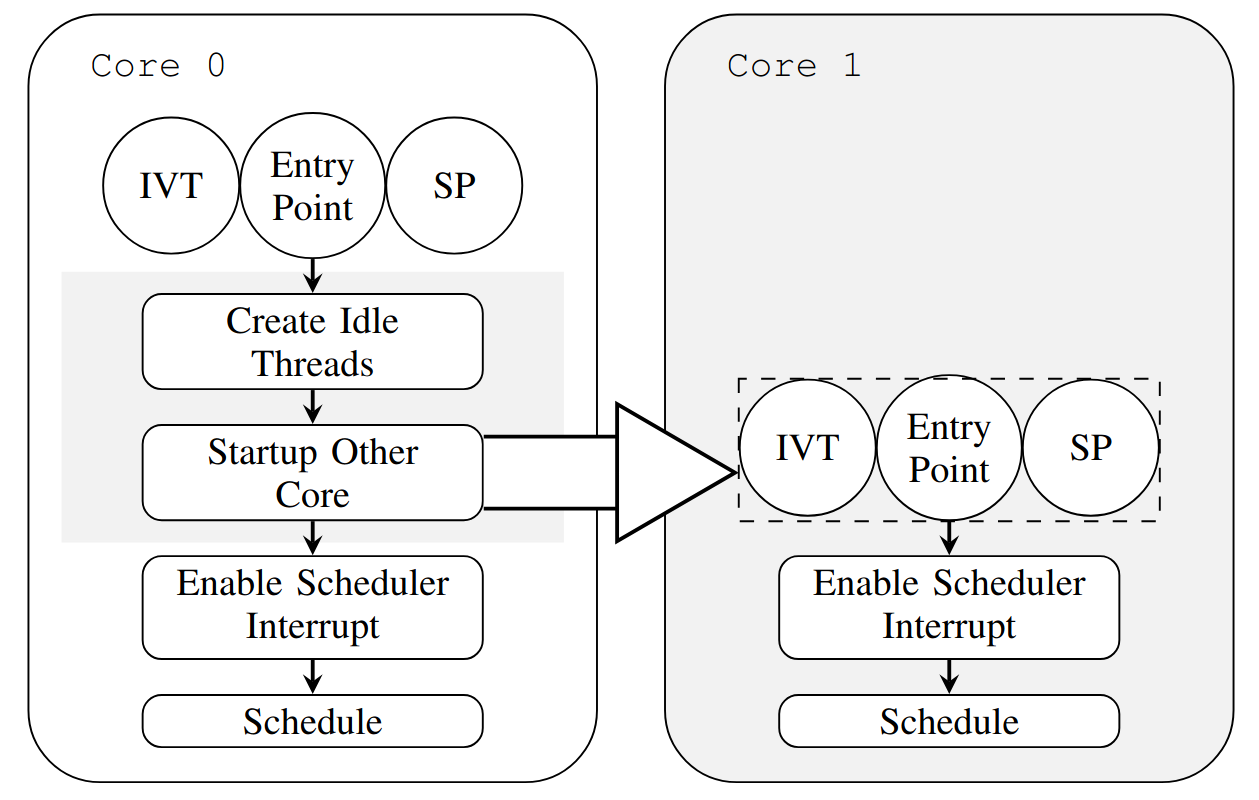
\includegraphics[width=0.95\columnwidth]{translate/figures/threading-startup-render-2.png}
     \caption{双核系统上的线程启动}
     \label{fig:startup}
 \end{figure}




\iffalse
\subsection{Idle Threads}

When a core is idle, it is prompted to enter low-power mode until the next thread is ready and waiting.
% Two alternative mechanisms are used to enter idle mode, depending on whether a system is single- or multicore. %\noteCA{``Two'' mechanisms?} 
On single-core, idle mode is entered in the scheduler exception, resulting in a lazy context switch (i.e. context is switched only when a different thread requires that). 
On multicore, however, such lazy context switching can result in race conditions, and thus idle threads are used instead.
% More in details: one idle thread is created per core during startup at the lowest priority.
% When no other thread is ready, the scheduler will execute this thread.
The idle threads execute at lowest priority and simply prompt the core to enter low-power mode until an interrupt occurs.
\fi

\subsection{全局调度方案}\label{sec:design:scheduling}


% \begin{itemize}
%     \item Two alternative designs: \textit{Global reallocation} routine (ThreadX) and \textit{Dynamic selection} (FreeRTOS, Nuttx, RT-Thread) approach
%     \begin{itemize}
%         \item 2-3 sentences each how they work on a high level
%     \end{itemize}
% \end{itemize}



% \OSname{} uses a global scheduling scheme.

% Global scheduling facilitates thread migration, where threads migrate between cores between executions.
% We chose global scheduling because it reduces context switches and priority inversions, and makes better use of the overall capacity~\cite{hardrealtime-multiprocessor-survey, brandenburg}.
% Furthermore, it avoids the thread allocation problem of partitioned scheduling, i.e., the problem of finding an optimal allocation of threads to cores.
% The main drawback of global scheduling is scalability, when the global runqueue becomes a bottleneck for context switching~\cite{EDF-RM-multiprocessor-survey}. However, this issue is negligible on MCUs --- which have a low processor count.
\OSname{} 使用全局调度方案

全局调度支持线程迁移,允许线程在执行过程中在不同核心之间动态移动。我们选择全局调度,是因为它能够有效减少上下文切换的频率,降低优先级反转的风险,并且更高效地利用整体计算资源~\cite{hardrealtime-multiprocessor-survey, brandenburg}。此外,全局调度还避免了分区调度中常见的线程分配难题,即如何为每个核心找到最优的线程分配方案。全局调度的主要缺点是其在可扩展性方面的局限性,尤其是在全局运行队列可能成为上下文切换瓶颈的情况下~\cite{EDF-RM-multiprocessor-survey}。然而,在微控制器场景中,由于处理器核心数量通常较少,这一问题的影响几乎可以忽略不计。


% \subsection{Assigning Threads to Cores}
% \label{sec:Assigning-Threads-to-Cores}
% With the single-core configuration, the thread-selection process simply reads the head of the runqueue. 
% However, on multicore, this would result in the same thread being executed on multiple cores.
% There are various approaches for selecting the next thread that a core should execute.
% We initially designed our scheduler so that it can accommodate either \textit{core reallocation} or alternatively \textit{dynamic thread selection} (see \autoref{sec:multicore-sched}). We then implemented both, before reporting on their performance on different hardware in \autoref{sec:benchmarks}.
\subsection{线程分配到核}
\label{sec:Assigning-Threads-to-Cores}
在单核配置中,线程选择过程仅需读取运行队列的头部。然而,在多核配置下,这种简单的选择方式会导致同一个线程在多个核上被执行。为了避免这种情况,我们探索了多种线程分配策略。我们最初设计的调度器能够灵活支持 \textit{核重分配} 或 \textit{动态线程选择}(参见 \autoref{sec:multicore-sched})。此后,我们不仅实现了这两种方法,还在 \autoref{sec:benchmarks} 中详细报告了它们在不同硬件平台上的性能表现。
%in our multicore effort in order to make an informed decision for our final implementation.

%  \begin{figure}[b]
%      \centering
%      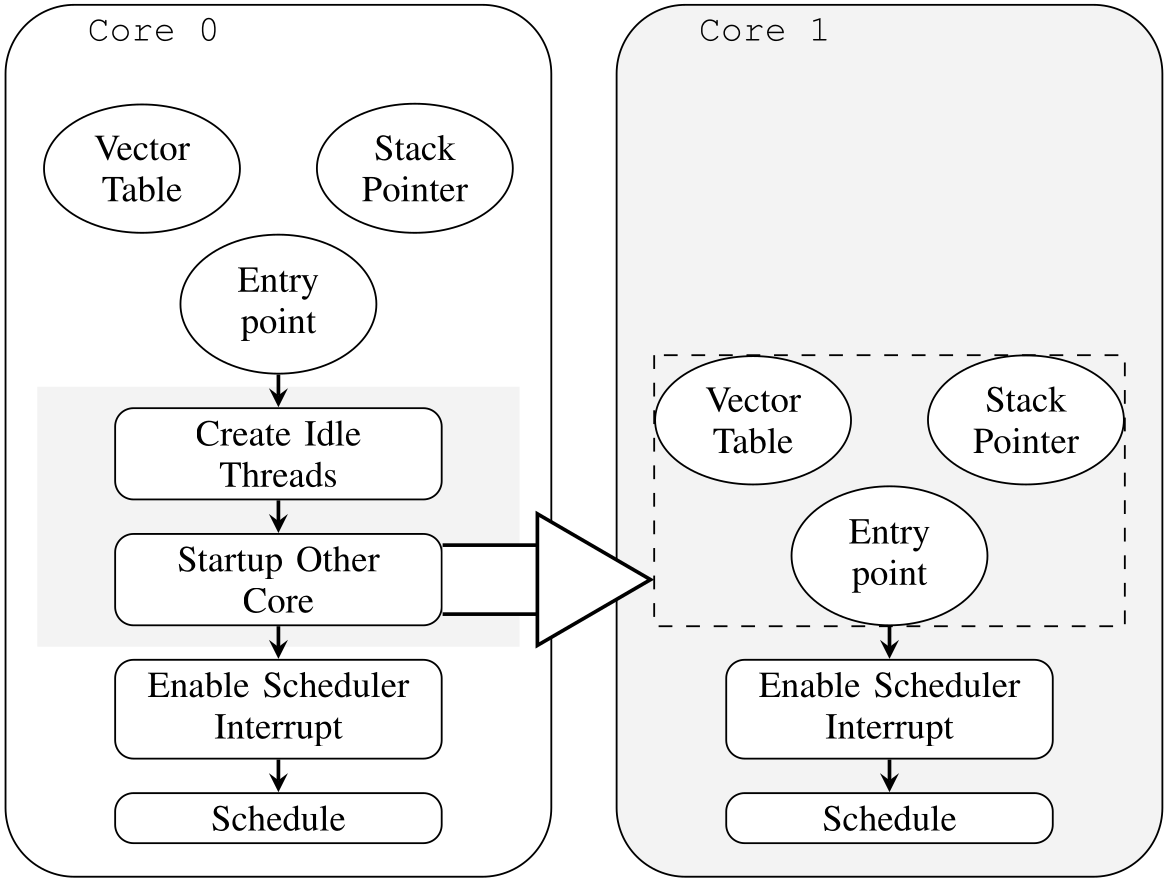
\includegraphics[width=\linewidth]{figures/threading-startup-render.png}
%      \caption{Threading startup on a dual-core system.}
%      \label{fig:startup}
%  \end{figure}

\iffalse
\subsubsection{Core Reallocation}

With this approach, a \textit{reallocation} routine maps the \textit{n} highest priority threads to the \textit{n} cores.
The allocation for each core is stored in an array that the scheduler interrupt handler reads upon invocation.
After each change in the runqueue, the \textit{reallocation} routine is executed.
It compares the previous allocation with the current highest priority threads in the runqueue, and updates the core allocation list with the goal of minimizing changes, and thus thread migration.
Based on the allocation changes, the routine returns the ID of the core where a context switch is needed.
A prominent example that follows this design is the ThreadX operating system.

\subsubsection{Dynamic Thread Selection}

In an alternative approach, implemented in FreeRTOS, NuttX, Zephyr or RT-Thread, the next thread for a core is selected directly from the runqueue by the scheduler interrupt handler upon invocation.
The thread is then removed from the runqueue to prevent it from being selected for multiple cores.
Conversely, when a running thread is preempted, it is re-added to the runqueue.
The scheduler uses the information it has readily available about thread state changes to trigger a scheduler interrupt on the specific core where a context switch is needed.
For instance, if a high-priority thread becomes ready, the scheduler interrupt is set for the core that is currently executing the lowest-priority thread.

\fi

% In an alternative approach, the scheduler selects the next thread for a core, in a dynamic fashion, upon invocation.
% The global scheduler uses the information it has readily available about changes in thread state changes, in the runqueue changes, to invoke the scheduler on the specific core where a context switch is needed.
% \noteEB{I attempted reformulation because it was difficult to parse. But somehow it is *still* difficult to parse. In particular, if there is a global scheduler, it should not sound suddenly like there are multiple schedulers...}
% The scheduler then %reads the next thread from the runqueue and 
% removes the thread from the runqueue, to prevent the same thread from being selected for multiple cores.
% Conversely, when a running thread is preempted, it is re-added to the runqueue.
% \subsection{Core Affinity Masks}

% Core affinities are a feature that allows pinning a thread so it runs on some specified core(s) only. %one or multiple specific cores. 
% This provides the user with fine-grained control over how and where threads may run. 
% % For example, core affinities can be used to bind two threads with different priorities to the same core, which will ensure that they can not run in parallel, and thus mutual exclusion between them.
% Core affinities are realized with a bitmask, where a set bit encodes that the thread can run on the core with this index. 
% The scheduler uses this information when selecting the core on which a thread should run.

\subsection{核亲和性掩码}

核亲和性是一种特性,允许将线程固定到特定的核上运行。这为用户提供了对线程运行位置和方式的精细控制。

核亲和性通过位掩码实现,其中设置的位表示线程可以在该索引对应的核上运行。调度器在选择线程应运行的核时会使用这些信息

% \subsection{Dynamic Priorities and Priority Inheritance}

% Thread priorities in \OSname{} can be changed dynamically at runtime for all active threads.
% A change in priority may result in a context switch if a running thread's priority is decreased or if a waiting thread's one increased.
% Furthermore, dynamic priorities facilitate priority inheritance for mutexes.
% If a higher-priority thread is blocked on a mutex that is currently owned by a lower-priority thread, the owning thread inherits the higher priority of the waiting thread.
% This prevents the owner from being preempted by other lower-priority threads 
% and thus helps avoid priority inversions caused by indirect blocking.

\subsection{动态优先级与优先级继承}

在 \OSname{} 中,所有活动线程的优先级都可以在运行时动态调整。如果运行中的线程优先级被降低,或者等待中的线程优先级被提高,这可能会触发上下文切换。此外,动态优先级还支持互斥锁的优先级继承。当一个高优先级线程因等待一个当前由低优先级线程持有的互斥锁而阻塞时,持有互斥锁的线程将继承等待线程的较高优先级。这可以防止持有者被其他低优先级线程抢占,从而有助于避免由间接阻塞引起的优先级反转问题。

% \subsection{Synchronization in the Scheduler\label{sec:design:sync}}

% \OSname{} implements mutual exclusion in the kernel through a global critical section, effectively resulting in a \textit{Big Lock} design.
% Thus, there is no concurrency in the kernel, which is tolerable given that such operations in \OSname{} are short.
% It ensures correctness, prevents data races and deadlocks, and simplifies operations that involve multiple data structures, such as the runqueue and Thread Control Blocks (TCBs), because no individual locking is needed.
% On single-core systems, it is sufficient to mask all interrupts to create a critical section.
% In multicore systems, an additional global spinlock is required to ensure that even threads on other cores cannot enter another critical section. 

\subsection{调度器中的同步\label{sec:design:sync}}

\OSname{} 通过全局临界区在内核中实现互斥,这实际上形成了一种 \textit{大锁} 设计。
因此,在内核中不存在并发问题,鉴于 \OSname{} 中此类操作的持续时间较短,这种设计是可以接受的。
它确保了操作的正确性,防止了数据竞争和死锁,并且简化了涉及多个数据结构的操作,例如运行队列和线程控制块(TCBs),因为无需单独锁定。
在单核系统中,屏蔽所有中断就足以创建一个临界区。
在多核系统中,需要额外的全局自旋锁来确保其他核心上的线程也无法进入另一个临界区。

% \subsection{Combining Scheduled Threads \& Async Rust Tasks}\label{sec:design:async}

% \OSname{} uses async code based on \emph{Embassy}~\cite{embassy} for system initialization and in the HAL.  
% There is always a system executor for async tasks. 
% Using the preemptive scheduler --- and thus threading --- is optional. 
% If the scheduler is not used, the system executor will run in interrupt context. 
% If the scheduler is used, the system executor executes in a thread. 
% Additional executors can be started in other threads. 
% When all tasks on an executor are pending, the owning thread is suspended. 
% Threads can block on async functions and wait for async resources from an executor.
% Thus, the gap is bridged between the scheduler, async Rust, future-based concurrency, and asynchronous I/O.

\subsection{调度线程与异步 Rust 任务结合}\label{sec:design:async}

\OSname{} 使用基于 \emph{Embassy}~\cite{embassy} 的异步代码进行系统初始化和硬件抽象层(HAL)的实现。
系统中始终存在一个用于执行异步任务的系统执行器.
使用抢占式调度器以及由此产生的线程是可选的。如果未使用调度器,系统执行器将在中断上下文中运行。如果使用了调度器,系统执行器则会在一个线程中执行。额外的执行器可以在其他线程中启动。当某个执行器上的所有任务都处于挂起状态时,拥有该执行器的线程将被挂起。线程可以阻塞在异步函数上,并等待来自执行器的异步资源。
因此,\OSname{} 在调度器、异步Rust、基于future的并发以及异步I/O之间架起了桥梁。




% 
% DRAFT THAT FIRST: Goals (and non-goals) in conjunction with benchmarks planned
% (with starting point: single-core scheduler is like RIOT-rs scheduler)


% - discussion of scheduler variants:
%    - mentioned that we face crossroad/ two avenues; shortly discuss them
%    - we tested them on two platforms; compare in one benchmark, max two
%    - reduced
%    - "present thesis in two minutes"
%    - describe all feature

\section{\OSname{} 调度器实现}

% \begin{itemize}
% \item Supported multicore platforms: RP2040, ESP32-S3, (multicore RISC-V is WIP)
% \end{itemize}

% As of this writing, \OSname{} supports multicore scheduling on three popular hardware platforms/architectures: the RP2040 and RP2350 (dual-core ARM Cortex-M0+/ dual-core ARM Cortex-M33 resp.) and the \espsthree{} (dual-core Xtensa LX7). RISC-V multicore scheduling support in \OSname{} is currently a work in progress. %As our approach is portable by design, we expect RISC-V multicore scheduling support (e.g. on the Raspberry Pi Pico2) to be available soon. In the meantime, RISC-V is supported in single-core scheduling mode only. %and only on the ESP32 family for the time being. 

% The RP2040, RP2350, and the \espsthree{} are well supported in the Rust ecosystem: the former through the Embedded-Rust working group and the \verb|rp-rs| project, the latter directly by Espressif through the \verb|esp-hal| project.
% \OSname{} leverages this support in its implementation.
截至本文撰写之时,\OSname{} 已在三种主流的硬件平台/架构上实现了多核调度功能:RP2040 和 RP2350(分别为双核 ARM Cortex-M0+/ 双核 ARM Cortex-M33)以及 \espsthree{}(双核 Xtensa LX7)。目前,\OSname{} 对 RISC-V 的多核调度支持仍在开发中。%鉴于我们的方法在设计上具有可移植性,我们预计 RISC-V 的多核调度支持(例如在 Raspberry Pi Pico2 上)将很快推出。与此同时,RISC-V 仅支持单核调度模式。%并且目前仅在 ESP32 系列上支持。

RP2040、RP2350 和 \espsthree{} 在 Rust 生态中得到了良好的支持:前者通过 Embedded-Rust 工作组和 \verb|rp-rs| 项目获得支持,后者则通过 Espressif 的 \verb|esp-hal| 项目直接获得支持。
\OSname{} 在其实现中充分利用了这些支持。

% , and in the next sections we focus on describing \OSname{} multicore scheduling support for these different architectures/boards.

\subsection{硬件抽象}

% \begin{itemize}
%     \item Impact of Rust: traits \& generics; leverage ecosystem (Embassy, esp-hal)
% \end{itemize}

% One of the main objectives of our work is clear hardware abstraction and the reduction of platform-specific code.
% Adding support for another chip should be minimal effort, particularly when there is already chip support in the ecosystem.
我们工作的主要目标之一是实现清晰的硬件抽象以及减少特定平台的代码。当生态中已经存在对某个芯片的支持时,增加对该芯片的支持应当是一项轻而易举的任务。
% that can be leveraged.
% \pagebreak
% In \OSname{}, hardware abstraction occurs at two levels:

% \textit{CPU architecture abstraction ---} At this layer, the scheduler logic for a CPU architecture, e.g., Cortex-M, is implemented. 
% It involves all architecture-specific code to set up a thread stack, configure the exception used to trigger the scheduler, and the actual context-switching logic. 
    
% \textit{Chip-level abstraction ---} The platform-specific logic for SMP is implemented at this layer.
%     % Concretely, an implementation must specify the number of available cores and a method to read out the current core identifier. 
%     For multicore scheduling, two mechanisms are required,
%     \begin{enumerate*}[label=(\roman*)]
%     \item for starting up the other core(s), and 
%     \item for invoking the scheduler on a specific core
%     \end{enumerate*}. 
%     % The latter is needed because, on the above architectural layer, a scheduler invocation only targets the scheduler on the current core. 
%     % Indeed, \OSname{} scheduling logic requires that the scheduler of all cores can be triggered directly, because logic running on one core can affect the state of a thread that is running (or should be running) on another core.
% %\end{itemize}

% \OSname{} takes advantage of the Rust type system, by specifying the above abstractions as \emph{traits}~\cite{rust-book_traits}.
在 \OSname{} 中,硬件抽象发生在两个层面:

\textit{CPU 架构抽象 ——} 在这一层,实现了针对特定 CPU 架构(例如 Cortex-M)的调度器逻辑。它涵盖了设置线程栈、配置触发调度器的异常以及实际的上下文切换逻辑等所有与架构相关的代码。

\textit{芯片级抽象 ——} 在这一层,实现了特定平台的对称多处理(SMP)逻辑。

对于多核调度,需要两种机制:
\begin{enumerate}[label=(\roman*)]
    \item 用于启动其他核心(或多个核心);
    \item 用于在特定核心上调用调度器。
\end{enumerate}

\OSname{} 利用了 Rust 的类型系统,通过将上述抽象定义为 \emph{特性}(traits)~\cite{rust-book_traits} 来实现。
% that are then implemented by each platform.
% Compared to the alternative practice of simply duplicating function signatures for every platform, which is common, e.g., in hardware abstraction layers programmed in C, this design is more concise and ergonomic.
% Adding support for another platform in the scheduler only requires two traits -- one per layer -- to be implemented.
% As a result, the corresponding chip-level SMP implementations in \OSname{} are only 70 lines of Code (LOC) for the RP2040 and 66~LOC for the \espsthree{}.
在调度器中为另一个平台添加支持,仅需实现两个特性——每个层面各一个。
因此,在 \OSname{} 中,RP2040 的芯片级对称多处理(SMP)实现仅有 70 行代码,而 \espsthree{} 的实现则为 66 行代码。

\subsection{特定平台的调度逻辑}

% \noindent \textit{On the RP2040/RP2350 ---} The chip implements (in hardware) two FIFO queues between the physical cores, which are utilized by \OSname{} during startup and for scheduler invocations.
% During startup, Core 1 remains in sleep mode until it receives the vector table, stack pointer, and entry function through the FIFO queue, based on a fixed protocol.
% After startup, the FIFO queue is used to invoke the scheduler on the other core. 
% A received message will trigger an interrupt, where the handler will set the local scheduler exception.
\noindent \textit{在 RP2040/RP2350 上 ——} RP2040/RP2350 芯片在硬件层面实现了两个 FIFO 队列,用于连接两个物理核心。这些队列在 \OSname{} 的启动过程和调度器调用中发挥关键作用。在启动阶段,核心 1 保持睡眠模式,直到通过 FIFO 队列接收到向量表、栈指针和入口函数,这一过程遵循一个固定的协议。启动完成后,FIFO 队列用于在另一个核心上调用调度器。接收到的消息将触发一个中断,中断处理程序会设置本地调度器异常,从而启动调度过程。
% \noteEB{is message passing between threads etc; something that should be described/characterized at some level, before it pops up here? Should Fig. 1 include a FIFO on each core?}
% \noteEF{This specific section here concerns message passing between \textbf{Cores}, which is implemented in Hardware, and only on the RP2040. The ESP32-S3 doesn't implement such FIFO queues. Message passing between threads is possible through software channel, but I think that's othogonal to this section, and probably belongs into section \ref{sec:user-guide}?}

% \noindent \textit{On the ESP32-S3 ---} The chip does not implement any inter-processor communication channel.
% Instead, two different software-triggered CPU interrupts are used to invoke a scheduler on each core, respectively.
% Startup of the second core on the \espsthree{} is implemented by writing the address of the entry function into the boot address of Core 1, then resetting and unstalling the core.
% The entry function sets up the vector table address and the stack pointer for this core, and then runs our threading startup logic.

\noindent \textit{在 ESP32-S3 上 ——} 该芯片未实现任何处理器间通信通道。相反,它通过触发两个不同的软件中断来分别在每个核心上调用调度器。在 \espsthree{} 上启动第二个核的启动是通过将入口函数的地址写入核心 1 的启动地址,然后重置并解除该核心的停机状态来实现的。入口函数会设置该核的向量表地址和栈指针,随后运行我们的线程启动逻辑。

\subsection{中断处理}

% On the RP2040/RP2350, each core is equipped with its own ARM Nested Vectored Interrupt
% Controller (NVIC). 
% On the \espsthree{}, each core has its own configurable interrupt matrix. 
% On both chips, nested interrupts are supported, so that a lower-priority interrupt can be preempted by a higher-priority one.
% External interrupts are routed to both cores,
% but only enabled on one core for handling, as described below.
在 RP2040/RP2350 上,每个核心都配备了各自的 ARM 嵌套向量中断控制器(NVIC)。
在 \espsthree{} 上,每个核心都有其可配置的中断矩阵。
在两种芯片上,都支持嵌套中断,使得低优先级的中断可以被高优先级的中断抢占。
外部中断被路由到两个核心,但仅在一个核心上启用以进行处理,具体如下所述。

% During startup, peripherals are initialized either in interrupt mode on Core 0 before threading is started, or by one high-priority thread. % whose core affinity can optionally be set.
% This initialization configures and enables the required interrupts on the core it executes on, which will then be the core that handles the related interrupts.

% Still, both cores share the same interrupt vector table, so it is also possible to manually mask and unmask interrupts on individual cores to configure where an interrupt should be handled.
在启动期间,外设初始化要么在核心 0 上以中断模式进行,且在启动线程之前完成,要么由一个高优先级线程完成。% 其核心亲和性可以可选地设置。
这种初始化会在其执行的核心上配置并启用所需的中断,而该核心随后将负责处理相关的中断。

尽管如此,两个核心共享同一个中断向量表,因此也可以手动在各个核心上屏蔽和解除屏蔽中断,以配置中断的处理位置。

\subsection{调度器中的同步}

% The scheduler is implemented through a single structure that contains the runqueue, TCBs, and other scheduling data, and implements all scheduling logic.
% This structure is protected by a wrapper type that ensures that all accesses to the scheduler are executed inside a critical section and that no reference to the scheduler can be obtained outside of it.
调度器通过一个单一结构实现,该结构包含运行队列、线程控制块(TCBs)以及其他调度数据,并实现了所有调度逻辑。
该结构被一个包装类型保护,确保所有对调度器的访问都在临界区中执行,并且无法在临界区之外获得对调度器的引用。
% Such access is realized in Rust closures~\cite{rust-book_closures},.
% that are provided with an immutable or mutable reference to the scheduler structure as input.
% The Rust compiler prevents the reference from being moved outside this closure in any way, thus access is only possible for the duration of the closure and therefore only while inside the critical section.

\iffalse
\subsection{Lock Guards}

Lock guards are common design pattern for synchronization primitives and mutual exclusion in Rust.
In case of \OSname{}, lock guards are used in both the \verb|critical-section| crate~\cite{critical-section} that \OSname{} is using, as well as \OSname{}'s own mutex implementation.
% ~\noteEB{Link/ref to crate? And: it struck me that some readers might not know what a "crate" is. (i) what doc should we cite on crates? (ii) where should we "introduce" the notion of crate? I get the feeling "crate" should be hinted at way before this stage. Maybe in section 2, e.g. mention that we aim to "take full advantage of Rust specificity beyond memory safety, for instance the crate system, and trait zero-cost abstractions"?}
The implementation takes advantage of Rust's ownership concepts and scoping rules for ergonomic and fail-safe lock usage. The life time of a lock guard corresponds to the time a lock is held.
On one hand, lock guards ensure that an acquired lock or critical section is always released again, even in case of code panics. On the other hand, lock guards facilitate access to the protected data – in Rust, synchronization primitives like mutexes typically own the data they protect. %\noteKS { @Elena please double check this is not cutting too much}
\fi
\iffalse 
where each variable has exactly one owner, which may be, for example, the function it is declared in.
If the variable goes out of scope, e.g., because the function returns, the variable is destructed and its memory freed.
However, before doing so, the destructor will call a \verb|drop| function first on the type itself, and then recursively on all its inner types. 
This \verb|drop| function can be implemented by the crate that defines the type, to add logic that should run just before the type is destructed.

In the case of lock guards, the \verb|drop| function is implemented to release the associated lock, and more precisely, this is also \textit{the only way to release a lock}.
If the lock should be released before the guard would usually go out of scope, it can be dropped manually, after which the guard is no longer accessible.
Thus, there is no way the protected inner data is accidentally accessed after the lock was already released.


\noteEF{Koen noted that this section may not be relevant/ interesting to the user. Purpose was to show how Rust impact the implementation of synchronization primitives and the gain from that. But if we're short on space, maybe remove this section?}
\noteEB{Let's first try to make it shorter, and tighten the rest too. Remove in last resort. Rust specifics = good}

% - mention stuff that specific to embedded Rust in that context
%    - discuss challenged and opportunities that come from Rust
\fi
\section{使用 \OSname{} 多核的微基准测试}
\label{sec:benchmarks}


% We next evaluate the performance of \OSname{} on popular hardware. We published our benchmark code in~\cite{ariel-benchmarks}. 

% The \textbf{dual-core MCUs} we used are:
% \begin{enumerate*}[label=(\roman*)]
% \item Espressif \espsthree{} with dual Xtensa LX7 at 240 MHz, and 
% \item RP2040/RP2350 with dual Cortex-M0+/M33 at 133/150 MHz.
% \end{enumerate*}


% The \textbf{single-core boards} we used for comparison are:
% \begin{enumerate*}[label=(\roman*)]
% \item a Nordic nRF52840 with a Cortex-M4 at 64 MHz, and 
% \item an Espressif \espcthree{} with a RISC-V RV32IMC at 160 MHz.
% \end{enumerate*}
接下来,我们在主流的硬件平台上评估了 \OSname{} 的性能。我们的基准测试代码已发布在~\cite{ariel-benchmarks}。

我们使用的\textbf{双核 MCU}包括:
\begin{enumerate}[label=(\roman*)]
\item Espressif \espsthree{},配备双核 Xtensa LX7,主频 240 MHz;
\item RP2040/RP2350,配备双核 Cortex-M0+/M33,主频分别为 133 MHz 和 150 MHz。
\end{enumerate}

我们用于对比的\textbf{单核开发板}包括:
\begin{enumerate}[label=(\roman*)]
\item Nordic nRF52840,配备 Cortex-M4,主频 64 MHz;
\item Espressif \espcthree{},配备 RISC-V RV32IMC,主频 160 MHz。
\end{enumerate}
%\footnote{The benchmarks are available at \url{https://github.com/elenaf9/RIOT-rs-benchmarks}. The used commit revision is \textit{TODO}.} that compare the scheduler performance, quantify the speedup, and ...(\textit{TBC}).
\iffalse
We measured performance on the following popular boards, commercially available off-the-shelf: 
\begin{itemize}
    \item Nordic nRF52840: Arm Cortex\nobreakdash-M4, single-core, 64 MHz, 256 KB RAM, 1 MB Flash memory;
    \item Espressif \espcthree{}: RISC\nobreakdash-V RV32IMC, single-core, 160 MHz, 400 KB SRAM, 4 MB Flash memory;
    \item Espressif \espsthree{}: Xtensa LX7, dual-core, 240 MHz, 8 MB RAM, 16 MB Flash memory;
    \item RaspberryPi Pico: Arm Cortex\nobreakdash-M0+, dual-core,  133 MHz, 264 KB SRAM, 2 MB Flash memory.
\end{itemize}
\fi

% On Xtensa and Cortex-M, the performance is measured in ticks.
在 Xtensa 和 Cortex-M 架构上,性能是通过时钟周期(ticks)来衡量的。
\iffalse
\begin{itemize}
    \item Cortex-M: SysTick timer with the processor clock as the clock source
    \item Xtensa: CCOUNT cycle count registers
    % \item RISC-V: \noteEF{Unfortunately we can't measure the performance in ticks on the ESP32-C3 or ESP32-C6, because the \textit{mcycle} register isn't implemented on RV32IMC... Instead we have to use the system timer at 16Mhz... do we even need benchmark data for a second single-core board?}
\end{itemize}
\fi
% On the RISC-V-based \espcthree{}, we instead use the system timer, which runs at 16 MHz.
% The measurements we present are the average of 1000 runs.
在基于 RISC-V 的 \espcthree{} 上,我们使用系统定时器进行测量,该定时器运行频率为 16 MHz。
我们所展示的测量结果是 1000 次运行的平均值。
%, at 10\%  of the processor clock speed.
%Each benchmark consists of one or multiple threads, configured at the lowest priority, of which one executes the benchmark function.
% Results were deemed valid only if no timer/counter wrap-around and no thread migration of the benchmark-thread happened.% wrap, and the benchmarking thread didn’t migrate between cores. 



\subsection{比较多核调度器的差异}

%We compare the scheduler performance of the two global multicore scheduler implementations discussed in \ref{sec:design:scheduling} on dual-core platforms with each other, and against the baseline RIOT-rs scheduler. For this, a simple benchmark was implemented where two pairs of threads alternate in waking each other and then suspending their own execution by setting and waiting for thread flags. Hence, the benchmark largely consists of context switches.
% \autoref{fig:flags} depicts micro-benchmarks in which four threads, grouped into pairs, alternate in waking each other up and then suspending their own execution. % by setting and waiting for thread flags (hence the cost of context switches dominates here). 
% We compare the performance of different variants of the scheduler: (i) the \emph{single-core} variant described in \autoref{sec:single-core}, (ii) a multicore variant using \emph{core reallocation}, and (iii) a multicore variant using \emph{dynamic thread selection} as mentioned in \autoref{sec:Assigning-Threads-to-Cores}. 

\autoref{fig:flags} 展示了一个微基准测试,其中四条线程被分为两组,交替唤醒对方并挂起自己的执行。% 通过设置和等待线程标志(因此上下文切换的成本在这里占主导地位)。
我们比较了不同调度器变体的性能:(i) 在 \autoref{sec:single-core} 中描述的 \emph{单核} 变体,(ii) 使用 \emph{核重分配} 的多核变体,以及 (iii) 在 \autoref{sec:Assigning-Threads-to-Cores} 中提到的使用 \emph{动态线程选择} 的多核变体。


\pgfplotstableread[col sep=comma,]{translate/data/flags_dual-core_espressif-esp32-s3-devkitc-1.csv}\flagsdualesp{}
\pgfplotstableread[col sep=comma,]{translate/data/flags_dual-core_rpi-pico.csv}\flagsdualpico{}
\pgfplotstableread[col sep=comma,]{translate/data/flags_dual-core_rpi-pico2.csv}\flagsdualpicotwo{}
\begin{figure}[t!]
     \begin{subfigure}[t]{0.49\columnwidth}
     \begin{tikzpicture}
         {
            \begin{axis}[
            ybar,
            ourybarstyle,
            bar width=8pt,
            enlarge x limits=0.2,
            height=4cm, width=\textwidth,
            ylabel={Ticks},
            ytick distance=1000,
            symbolic x coords={{Single Core},{Multicore (Reallocation)},{Multicore (Dynamic)}},
            xticklabels={{Single Core},{Multicore\\(Reallocation)},{Multicore\\(Dynamic)}},
            nodes near coords style={font=\small, black, rotate=70, anchor=south east, yshift=-6pt, xshift=+27pt},
            xticklabel style={font=\small, rotate=45, anchor=east, align=right},
        ]
      \addplot table [y index=1]{\flagsdualpico};
      \addplot table [y index=1]{\flagsdualpicotwo};
    \end{axis}}
    \end{tikzpicture}
    \caption{RP2040/RP2350 (blue/purple)\label{fig:flags_rp2040}}
     \end{subfigure}
     \begin{subfigure}[t]{0.49\columnwidth}
     \begin{tikzpicture}
         {
            \begin{axis}[
            ybar,
            ourybarstyle,
            bar width=15pt,
            enlarge x limits=0.2,
            height=4cm, width=\textwidth,
            ylabel={Ticks},
            ytick distance=1000,
            symbolic x coords= {{Single Core},{Multicore (Reallocation)},{Multicore (Dynamic)}},
            xticklabels={{Single Core},{Multicore\\(Reallocation)},{Multicore\\(Dynamic)}},
            nodes near coords style={font=\small, black, rotate=45, anchor=south west, xshift=-2pt},
            xticklabel style={font=\small, rotate=45, anchor=east, align=right},
        ]
      \addplot table [y index=1]{\flagsdualesp};
    \end{axis}}
    \end{tikzpicture}
    \caption{ESP32-S3 (dual Xtensa LX7)\label{fig:flags_esp32s3}}
    \end{subfigure}
    \caption{两种多核调度器设计的上下文切换性能与单核配置的对比 \label{fig:flags}}
\end{figure}

% The results show that \textit{dynamic} outperforms \textit{reallocation} on all the multicore microcontrollers we tested.

% The results show that \textit{dynamic} outperforms \textit{reallocation} on both microcontrollers we tested. 
% The relatively more complex \textit{reallocation} routine, executed after each thread state change, takes a toll. 
% We notice a degradation of the performance of \textit{reallocation} versus single-core on RP2040, whereas speedups are observed on \espsthree{}. %This can be explained by different degrees of parallelization on the two platforms.

结果表明,在我们测试的所有多核微控制器上,动态分配优于重新分配。相对复杂的重新分配例程在每次线程状态变化后执行,会带来一定的代价。

\iffalse
\begin{enumerate}
    \item The \textit{Dynamic} approach outperforms the \textit{Reallocation} on both platforms.
    \item On the RP2040, no significant speedup was achieved through the multicore configuration, and even a degradation in case of the \textit{Dynamic} approach. On the \espsthree{}, the speedup is a factor of 1.3 in the \textit{Reallocation} approach and 1.5 for the \textit{Dynamic} one.
\end{enumerate}
\fi
%(1) is likely due to the complexity of the \textit{reallocation} routine, which is executed after each thread state change. The findings in (2) can be explained by different degrees of parallelization on the two platforms.
%As discussed in \autoref{sec:design:sync}, \OSname{} applies mutual exclusion to the whole kernel, and thus %no parallelization in the scheduler is possible.
% The benchmark largely consists of scheduler operations. Thus, mutual exclusion in the scheduler forces mostly sequential execution on the RP2040.
% In contrast, on the \espsthree{}, parallelization happens differently in hardware, forcing sequential execution less often. %however, 
% Furthermore, one benchmark iteration on \espsthree{} requires
% many more ticks than on the RP2040.
% Thus, \espsthree{} reaps more benefits from parallelization in this benchmark.
% %If we assume that this can be at least partly 
% %linked to a larger cost of the scheduler interrupt (and the saving and restoring of the trap frame). Thus, this larger segment that can run independently between the cores on this platform reaps more benefits from parallelization.
% In the following, we focus on the \textit{dynamic thread selection} variant for our multicore scheduling.
该基准测试主要由调度器操作构成。因此,RP2040上的调度器互斥机制导致其主要以顺序方式执行。
相比之下,在\espsthree{}上,硬件层面的并行化机制有所不同,较少强制执行顺序操作。此外,\espsthree{}上完成一次基准测试迭代所需的时钟周期远多于RP2040。因此,在此基准测试中,\espsthree{}能够从并行化中获得更多优势。
接下来,我们将重点关注多核调度中的\textit{动态线程选择}结构。
%approach, which we study further in the following.
% for our final SMP implementation. We furthermore found this approach to be the simpler and more intuitive one of the two, although additional care must be taken due to the lack of a global state. The following subsections use the \textit{dynamic} scheduler implementations for multicore.

% \iffalse
% \begin{figure}[htbp]
%      \begin{subfigure}[t]{0.49\columnwidth}
%     \centering
%          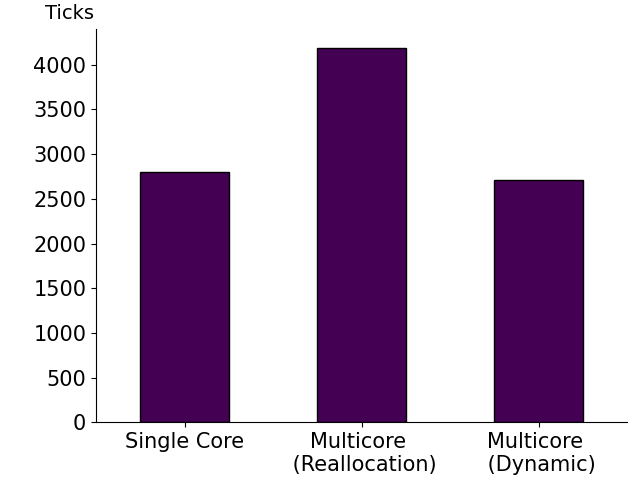
\includegraphics[width=\textwidth]{figures/flags_dual-core_rpi-pico.png}
%          \caption{RP2040 (dual Cortex-M0+)\label{fig:flags_rp2040}}
%      \end{subfigure}
%      \hfill
%      \begin{subfigure}[t]{0.49\columnwidth}
%          \centering
%          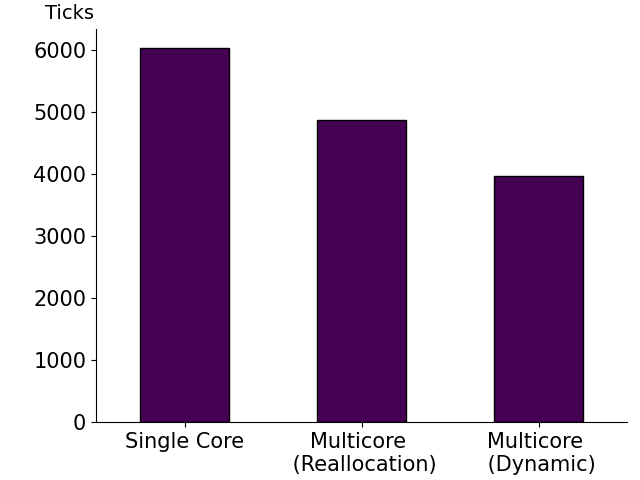
\includegraphics[width=\textwidth]{figures/flags_dual-core_espressif-esp32-s3-wroom-1.png}
%          \caption{ESP32-S3 (dual Xtensa LX7)\label{fig:flags_esp32s3}}
%      \end{subfigure}
%     \caption{Context switching performance of the two multicore scheduler designs compared with single-core configuration~.\label{fig:flags}}
% \end{figure}
% \fi
\subsection{多核调度的开销}

% We next measure
% the overhead of our multicore scheduling feature, compared to the single-core scheduler we started from in \autoref{sec:single-core}.
% For this, we focus on thread preemption, because, compared to single-core, the multicore feature adds an additional step: inserting the preempted thread back into the runqueue. %, whereas in the case of single-core this step is skipped.
% \autoref{fig:preempt} reports on micro-benchmarks performed on different single-core boards, in which a lower-priority thread sets the flag for a higher-priority thread, resulting in a context switch.

% We observe that the overhead when the multicore feature is enabled remains quite small, approx. 9.6\% on the nRF52840 and 5.3\% on the \espcthree{}. 
% Conveniently, we can therefore enable multicore by default

% in \OSname{}.

接下来,我们测量多核调度功能的开销,并将其与我们在\autoref{sec:single-core}中开始时的单核调度器进行比较。为此,我们专注于线程抢占,因为与单核相比,多核功能增加了一个额外的步骤:将被抢占的线程重新插入运行队列。%而在单核情况下,此步骤会被跳过。
\autoref{fig:preempt}报告了在不同单核开发板上进行的微基准测试结果,其中低优先级线程设置了一个标志以触发高优先级线程的运行,从而导致上下文切换。
我们观察到,启用多核功能时的开销仍然很小,在nRF52840上约为9.6%,在\espcthree{}上约为5.3%。因此,我们可以在\OSname{}中默认启用多核功能。

\pgfplotstableread[col sep=comma,]{translate/data/preempt_both_ai-c3.csv}\preemptesp{}
\pgfplotstableread[col sep=comma,]{translate/data/preempt_both_nrf52840dk.csv}\preemptnrf{}
\begin{figure}[t!]
     \begin{subfigure}[t]{0.49\columnwidth}
     \begin{tikzpicture}
         {
            \begin{axis}[
            ybar,
            ourybarstyle,
            bar width=20pt,
            enlarge x limits=0.4,
            height=4cm, width=\textwidth,
            ylabel={Ticks},
            ytick distance=200,
            symbolic x coords={{Multicore scheduler disabled},{Multicore scheduler enabled}},
            xticklabels={{disabled},{enabled}},
            nodes near coords style={font=\small, black, rotate=45, anchor=south west, xshift=-2pt},
            xticklabel style={font=\small, align=center},
        ]
      \addplot table [y index=1]{\preemptnrf};
    \end{axis}}
    \end{tikzpicture}
         \caption{nRF52840 (Cortex-M4)\label{fig:preempt_nrf52840}}
     \end{subfigure}
     \begin{subfigure}[t]{0.49\columnwidth}
     \begin{tikzpicture}
         {
            \begin{axis}[
            ybar,
            ourybarstyle,
            bar width=20pt,
            enlarge x limits=0.4,
            height=4cm, width=\textwidth,
            ylabel={Ticks},
            ytick distance=50,
            symbolic x coords={{Multicore scheduler disabled},{Multicore scheduler enabled}},
            xticklabels={{disabled},{enabled}},
            nodes near coords style={font=\small, black, rotate=45, anchor=south west, xshift=-2pt},
            xticklabel style={font=\small, align=center},
        ]
      \addplot table [y index=1]{\preemptesp};
    \end{axis}}
    \end{tikzpicture}
         \caption{ESP32-C3 (RISC-V)\label{fig:preempt_esp32c3}}
    \end{subfigure}
    \caption{在单核硬件上测量的多核调度特性开销 %when a running thread is being preempted on a single-core board.
    \label{fig:preempt}}
\end{figure}
% \iffalse
% \begin{figure}[htbp]
%      \begin{subfigure}[t]{0.24\textwidth}
%          \centering
%          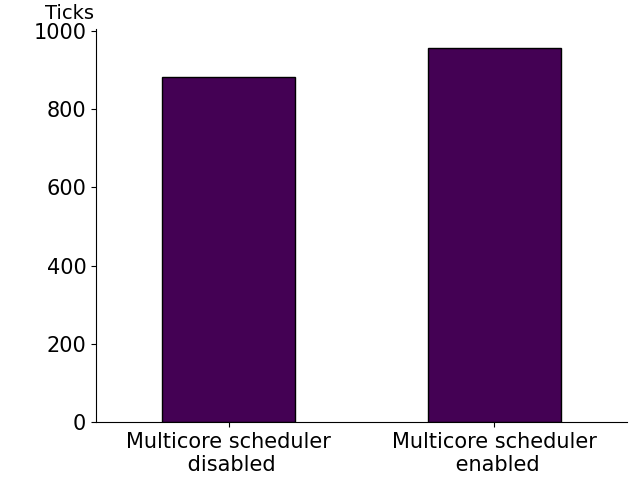
\includegraphics[width=\textwidth]{figures/preempt_both_nrf52840dk.png}
%          \caption{nRF52840 (Cortex-M4)\label{fig:preempt_nrf52840}}
%      \end{subfigure}
%      \hfill
%      \begin{subfigure}[t]{0.24\textwidth}
%          \centering
%          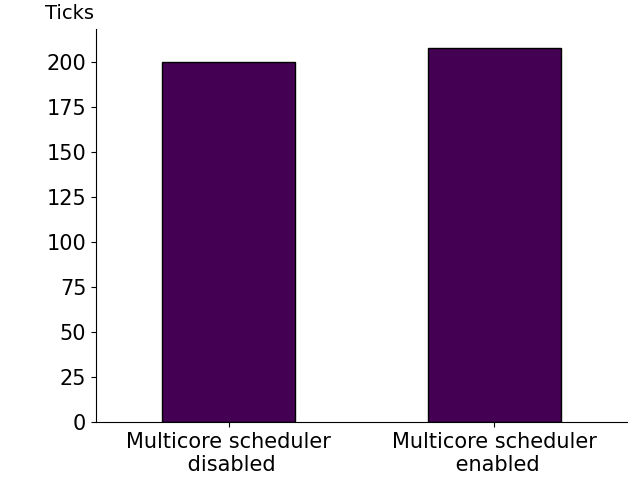
\includegraphics[width=\textwidth]{figures/preempt_both_ai-c3.png}
%          \caption{ESP32-C3 (RISC-V)\label{fig:preempt_esp32c3}}
%      \end{subfigure}
%     \caption{Overhead of the multicore scheduling feature when a running thread is being preempted.\label{fig:preempt}}
% \end{figure}
% \fi  

\subsection{计算密集型任务的加速}

\pgfplotstableread[col sep=comma,]{translate/data/matrix-mult_speedup_espressif-esp32-s3-devkitc-1.csv}\matrixesp{}
\pgfplotstableread[col sep=comma,]{translate/data/matrix-mult_speedup_rpi-pico.csv}\matrixpico{}
\pgfplotstableread[col sep=comma,]{translate/data/matrix-mult_speedup_rpi-pico2.csv}\matrixpicotwo{}
\begin{figure}[t]  
     \begin{subfigure}{0.49\columnwidth}
     \begin{tikzpicture}                                                   
         {
            \begin{axis}[                  
            ourlinestyle,              
            height=4cm, width=\textwidth,  
            ylabel={Relative speedup},     
            ytick distance=0.5,         
            tension=0.1,                
        ]                               
        \addplot+[myTeal, mark options={fill=myTeal}] table [x=0, y=speedup] {\matrixpico};                    
        \addplot+[myEggplant, mark options={fill=myEggplant}] table [x=0, y=speedup] {\matrixpicotwo};
    \end{axis}}                           
    \end{tikzpicture}      
     \caption{RP2040/RP2350 (blue/purple)\label{fig:matrix-mult_rp2040}}
     \end{subfigure}                                                   
     \begin{subfigure}{0.49\columnwidth}                                                                            
     \begin{tikzpicture}                                                                                                          
         {                                                                                                              
            \begin{axis}[                                                                                    
            ourlinestyle,                                                                             
            height=4cm, width=\textwidth,
            ylabel={Relative speedup},
            ytick distance=0.5,
        ]
        \addplot+[myTeal, mark options={fill=myTeal}] table [x=0, y=speedup] {\matrixesp};
    \end{axis}}             
    \end{tikzpicture}
         \caption{ESP32-S3 (dual Xtensa LX7)\label{fig:matrix-mult_esp32s3}}
    \end{subfigure}                                                             
    \caption{\(N\times N\) 矩阵的乘积, \(N\in\{10, 20, ...,  80\}\)\label{fig:matrix-mult}}
\end{figure}  
% We next benchmark 
% $N\times N$ matrix multiplication, with and without the multicore feature. 
% In the single-core configuration, the two computations are executed sequentially.
% For multicore, the tasks are distributed to two threads that are scheduled in parallel.
% We observe in Fig.~\ref{fig:matrix-mult} that when $N$ is small, IPC overhead dominates parallelization gains. When $N$ grows larger, we observe a performance gain tending towards 2x.
% We also notice that performance gains are not strictly linear. This is subject for further investigation --- it might be due to MCU-specific memory subsystem characteristics. %, subject to further investigation. 
% For example, on the RP2040, both cores compete for a shared memory bus~\cite{pico-mem-layout}.
接下来,我们分别在启用和未启用多核功能的情况下, 进行了 $N\times N$ 矩阵乘法的基准测试。在单核配置中,两次计算是顺序执行的。对于多核配置,任务被分配到两个线程中,并且这两个线程是并行调度的。
从图~\ref{fig:matrix-mult}中我们可以观察到,当 N 较小时,IPC(进程间通信)开销主导了并行化的收益。而当 N 增大时,我们观察到性能提升逐渐趋于 2 倍。我们还注意到性能提升并非严格线性增长。这有待进一步研究——它可能是由于 MCU(微控制器)特定的存储子系统特性所导致的。例如,在 RP2040 上,两个核会竞争共享的内存总线~\cite{pico-mem-layout}。
% \noteEF{For the record: It could still be that the speedup tends towards 2x if we test larger matrix sizes, e.g. 50x50. However, we can't do that with our benchmark because the timer wraps before the computation is completed.}

\textbf{总结 ---} 通过采用全局调度方案和优先级机制,我们实现了\emph{持续工作}和\emph{实时性}特性。我们的硬件抽象提供了\emph{可移植性},并且我们通过实验测量展示了\emph{透明性}。因此,我们已经实现了我们在第~\ref{sec:goals}节中设定的目标。
% \iffalse
% \begin{figure}[b!]
%      \centering
%      \begin{subfigure}[t]{0.24\textwidth}
%          \centering
%          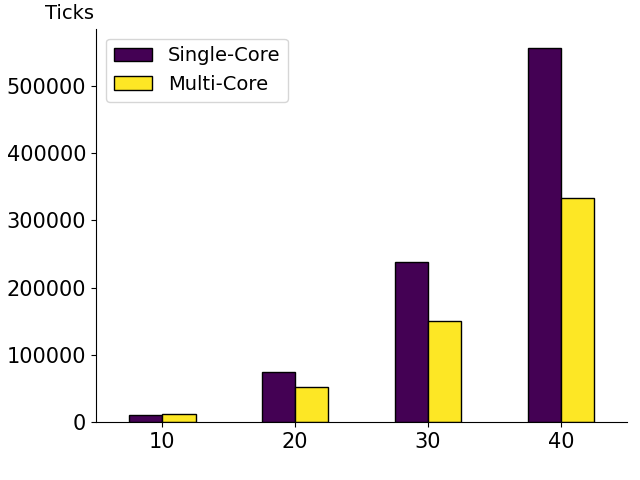
\includegraphics[width=\textwidth]{figures/matrix-mult_dual-core_rpi-pico.png}
%          \caption{RP2040\label{fig:matrix-mult_rp2040}}
%      \end{subfigure}
%      \hfill
%      \begin{subfigure}[t]{0.24\textwidth}
%          \centering
%          \includegraphics[width=\textwidth]{figures/matrix-mult_dual-core_espressif-esp32-s3-devkitc-1.png}
%          \caption{ESP32-S3\label{fig:matrix-mult_esp32s3}}
%      \end{subfigure}
%     \caption{Matrix-Multiplication performance of single- vs multicore for NxN matrices, \(N\in\{10, 20, 30, 40\}\)\label{fig:matrix-mult}}
% \end{figure}
% \fi
                             



%\textbf{Summary ---} Multicore scheduling overhead compared to a single-core scheduling variant is measurable but minor, thus the multicore variant can be the default on all platforms. In practice, parallel computation speedup with multicore scheduling is indeed substantial: we measured up to 175\% on dual core. \emph{Dynamic thread selection} outperforms other multicore variants, so we chose it as our default in \OSname{}. 
 %\noteEB{Kaspar TO DO: check the summary}
\section{Ariel 操作系统概述 %\& User Guide
}\label{sec:user-guide}

 \begin{figure}[t!]
     \centering
     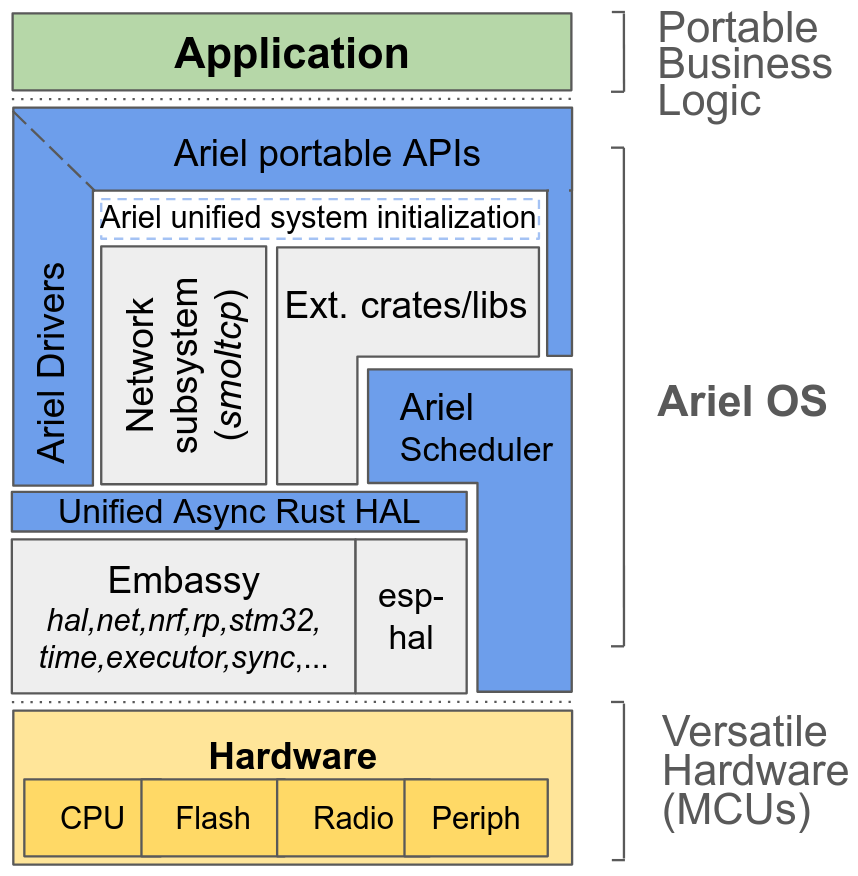
\includegraphics[width=0.7\linewidth]{translate/figures/arch-diagram-v4.png}
     \caption{\OSname{} 体系结构图%\noteCA{Ariel portable APIs also reach down to the Ariel scheduler; making it more closed and less fragmented. And this will need a color code legend.}
     }
     \label{fig:ariel-arch}
 \end{figure}
 

%\noteEB{Kaspar TO DO: choose a diagram ;)} \noteKS{I prefer EB's diagram, I tried to put in more embassy}
%Beyond its scheduler, \OSname{} aims to be a one-stop-shop for distributed computing and networked applications on heterogeneous 32-bit MCUs.
% \OSname{} is fully open-source~\cite{ariel-os-repo}. For basic hardware abstraction and async Rust programming, \OSname{} builds on top of Embassy~\cite{embassy}. Fig. \ref{fig:ariel-arch} shows how \OSname{} components (in blue) harness the ecosystem of embedded Rust (in grey).
% In particular, \OSname{} combines the following elements:
\OSname{}是完全开源的~\cite{ariel-os-repo}。对于基础硬件抽象和异步Rust编程,\OSname{}基于Embassy构建~\cite{embassy}。图\ref{fig:ariel-arch}展示了\OSname{}组件(蓝色部分)是如何利用嵌入式Rust生态系统(灰色部分)的。
具体来说,\OSname{}结合了以下元素:
%It tries to achieve that by increasing the level of abstraction, providing re-usable building blocks with usable defaults, better supporting diverse configurations in the build system, reducing boiler plate... higher level of abstraction makes high-level features possible ...
%\noteCA{… ``by providing convenient defaults for repetitive tasks of application developers''? (may be in a direction not useful for the audience, EB has opinion)}
\iffalse
\begin{itemize}
    \item Abstracting system initialization: system initialization is provided
    \item Unified peripheral APIs for application code portability: hardware access (sensor/actuator abstraction); network access (sock equivalent?). Code re-use of business logic across HW, e.g., our benchmarks code are completely HW-independent.
    \item Efficient code: automatic low-power mode exploitation; low memory footprint; zero-cost abstraction (exploiting Rust).
    \item Library OS: integration of curated set of drivers, crypto libs, network stacks. Various combinations/configs cover versatile use cases.
    \item Dependability: Rust inherent safeguards; Formal verification for critical modules (eg runqueue); 
    \item Networked: integrates IPv4 or IPv6, HTTP/TCP or CoAP/UDP network stacks over wireless/wired link layers, as well as network security standards (COSE, OSCORE, EDHOC, TLS...)
\end{itemize}
\fi

% \textbf{Versatile network stack configurations ---}
% \OSname{} integrates a network stack (\emph{embassy-net/smoltcp}~\cite{smoltcp}) combined with additional modules we provide allowing various network configurations. These configuration options include IPv4 and IPv6, HTTP/TCP and CoAP/UDP, over wireless and wired link layers, secured by open standards including COSE, OSCORE, EDHOC, TLS~\cite{tschofenig2019cyberphysical} and a curated set of libraries providing cryptographic backends.
\textbf{灵活的网络栈配置 ---}
\OSname{}集成了一个网络栈(\emph{embassy-net/smoltcp}~\cite{smoltcp}),并结合了我们提供的额外模块,支持多种网络配置。这些配置选项包括IPv4和IPv6、HTTP/TCP和CoAP/UDP,支持无线和有线链路层,并通过开放标准(包括COSE、OSCORE、EDHOC、TLS~\cite{tschofenig2019cyberphysical})以及精选的密码学后端库进行安全保护。

% \textbf{Abstracted system initialization ---}
% On MCUs, code initializing the system can be very challenging for developers. \OSname{} thus abstracts initialization, e.g., setting up
% \begin{enumerate}[label=(\roman*)]
% \item the network stack, 
% \item cryptographic material and identities, 
% \item the random number generator, 
% \item USB peripherals,
% \end{enumerate}
% etc. 
% Configuration is handled at build system level. Convenient defaults are provisioned. Boilerplate is thus minimized and high-level building blocks are provided to application logic. %\noteEB{Kaspar TODO: check/improve short version}
\textbf{抽象化的系统初始化 ---}
在微控制器(MCU)上,初始化系统的代码对开发人员来说可能极具挑战性。因此,\OSname{}对初始化过程进行了抽象化,例如设置:
\begin{enumerate}[label=(\roman*)]
\item 网络栈,
\item 密码学材料和身份,
\item 随机数生成器,
\item USB外设,
\end{enumerate}
等等。
配置在构建系统层面进行处理,并提供了方便的默认设置。这样可以最小化样板代码,同时为应用逻辑提供了高级构建模块。%\noteEB{Kaspar TODO: check/improve short version}

% \textbf{Unified peripheral APIs ---} 
% \OSname{} crafted peripheral initialization and setup (for GPIO, I2C, SPI accessing sensors/actuators) to be identical across MCU families. Thereby, application code written once can be compiled for all devices that \OSname{} supports. %Where MCU differences can not be hidden, they are made available in a way that maximizes portablility.
% This is a substantial improvement over the state of the art in embedded Rust (crates such as \emph{embedded-hal} or \emph{embedded-hal-async}) which leave out initialization, and thus lead to a jungle of initialization APIs --- and very limited application code portability. %\noteEB{Kaspar TODO: check/improve short version}

\textbf{统一的外设API ---}
\OSname{}设计了外设初始化和设置(针对GPIO、I2C、SPI访问传感器/执行器),使其在不同微控制器(MCU)系列中保持一致。因此,一次编写的应用程序代码可以编译到所有\OSname{}支持的设备上。%在无法隐藏MCU差异的地方,它们以最大化可移植性的方式提供。
这比嵌入式Rust的现有状态有了显著改进(例如\emph{embedded-hal}或\emph{embedded-hal-async}等crate),这些crate省略了初始化,从而导致了初始化API的混乱——以及非常有限的应用程序代码可移植性。%\noteEB{Kaspar TODO: check/improve short version}

% \textbf{Meta build system ---}
% The \OSname{} toolchain takes full advantage % of the large ecosystem of
% of the embedded Rust \emph{crates} ecosystem and the Rust build system \emph{Cargo}. To work around limitations w.r.t. extremely diverse modular target configurations, we wrapped Cargo in \emph{laze}~\cite{laze}, our meta-build system handling the huge matrix of software configurations on various boards.% We published the source code of \emph{laze} in~\cite{laze}.

\textbf{元构建系统 ---}
\OSname{}工具链充分利用了嵌入式Rust的\emph{crates}生态系统和Rust构建系统\emph{Cargo}。为了应对极其多样模块化的目标配置的限制,我们将Cargo封装在\emph{laze}~\cite{laze}中,这是一个元构建系统,用于处理各种开发板上庞大的软件配置矩阵。% 我们在~\cite{laze}中发布了\emph{laze}的源代码。

%With this landscape in mind, the remainder of the paper focuses primarily on the scheduler aspects.

\iffalse
In the embedded Rust ecosystem, the two interface-only crates `embedded-hal` and `embedded-hal-async` are the de-facto standard API for accessing an MCU's hardware peripherals like GPIO pins and I2C/SPI buses. While they enable GPIO/I2C/SPI peripherals to be used by e.g., drivers in an implementation agnostic way, the *initialization* and *setup* of the peripherals is intentionally left out of the traits in order to make them universally usable.
This leads to different `embedded-hal`(`-async`) implementations providing slightly or very different initialization APIs (\noteKS{reference embassy-hals, atsamd, esp-rs, ...?}
\OSname{} improves on this by providing a unified API for peripheral initialization that is designed to be identical across MCU families, allowing applications to be written once but compiled for all devices that \OSname{} supports. Where MCU differences can not be hidden, they are made available in a way that maximizes portablility. \noteKS{Mention frequency macro?}
\fi

% - present briefly \OSname{} as a whole with single core support (Basically RIOT-rs as it is/was), and claim explicitly as 
% - usage of Async Rust / Embassy?
% - library OS aspect
% - interaction with scheduler
% - add a brief architecture diagram 
%  (Basically: some kind of equivalent of https://inria.hal.science/hal-00945122/document (was for RIOT)
% \section{Conclusions}
% In this paper we introduced \OSname{}, the first embedded Rust operating system for microcontrollers supporting both single- and multicore preemptive scheduling combined with asynchronous Rust.
% We assessed experimentally how 
% a unique multicore scheduler can be the convenient default on all supported multicore platforms. 
% Still, applications 

% can opt out of multicore scheduling when parallelization is unneeded.

% \OSname{} thus enriches the set of available open source tools 
% for secure and efficient distributed computing applications involving sensors/actuators or small networked devices using 32-bit MCUs such as ARM Cortex\nobreakdash-M, RISC\nobreakdash-V, or ESP32.

\section{结论}
在本文中,我们介绍了\OSname{},这是第一个支持单核和多核抢占式调度以及异步Rust的微控制器嵌入式Rust操作系统。我们通过实验评估了在所有支持的多核平台上,独特的多核调度器如何可以作为便捷的默认选项。然而,当并行化并非必要时,应用程序可以选择退出多核调度。
因此,\OSname{}丰富了现有的开源工具集,适用于涉及传感器/执行器或使用32位微控制器(如ARM Cortex\nobreakdash-M、RISC\nobreakdash-V或ESP32)的小型网络设备的安全高效分布式计算应用。

%Researchers can use \OSname{} as common playground for experimental implementation and performance studies involving embedded Rust software on all the relevant 32-bit microcontroller architectures (ARM Cortex\nobreakdash-M, RISC\nobreakdash-V, ESP32).
%Industry users from diverse verticals can use \OSname{} to accelerate their transition from C/C++ towards safer embedded Rust, while benefiting from a high degree of hardware agility. %, ingrained by design. 
%\textbf{Code Availability ---} \OSname{} is fully open source~\cite{ariel-os-repo}.% and  maintained on a public git repository by 10+ people located in 4 countries across the European Union.

%in terms of reusing their software (business logic) on a wide variety of microcontroller architectures and commercially available off-the-shelf boards in this category.



% \bibliographystyle{translate/IEEEtran}
% \bibliography{translate/tlrefs.bib}



% 大量原本用C/C++实现的低级系统软件组件,目前正在被用Rust语言重新编写。Rust是一种相对更安全、更可靠的编程语言。然而,到目前为止,还没有用Rust编写的嵌入式操作系统支持微控制器上的多核抢占式调度。因此,本文填补了这一空白,提出了一个新的操作系统:Ariel OS。我们描述了它的设计,提供了其实现的源代码,并在主流的32位微控制器架构上进行了微基准测试,包括ARM Cortex-M、RISC-V和Espressif Xtensa。我们展示了我们的调度器如何在利用多核优势的同时,仅在单核硬件上产生极小的额外开销。正因如此,Ariel OS 为研究和行业从业者针对小型联网设备提供了一个便捷的嵌入式软件平台。


% \section{图表示例}

% \subsection{图}

% 附录中的图片示例(图~\ref{fig:appendix-translation-figure})。

% \begin{figure}
%   \centering
%   
\includegraphics[width=0.6\linewidth]{example-image-a.pdf}
%   \caption{附录中的图片示例}
%   \label{fig:appendix-translation-figure}
% \end{figure}


% \subsection{表格}

% 附录中的表格示例(表~\ref{tab:appendix-translation-table})。

% \begin{table}
%   \centering
%   \caption{附录中的表格示例}
%   \begin{tabular}{ll}
%     \toprule
%     文件名          & 描述                         \\
%     \midrule
%     thuthesis.dtx   & 模板的源文件,包括文档和注释 \\
%     thuthesis.cls   & 模板文件                     \\
%     thuthesis-*.bst & BibTeX 参考文献表样式文件    \\
%     thuthesis-*.bbx & BibLaTeX 参考文献表样式文件  \\
%     thuthesis-*.cbx & BibLaTeX 引用样式文件        \\
%     \bottomrule
%   \end{tabular}
%   \label{tab:appendix-translation-table}
% \end{table}


% \section{数学公式}

% 附录中的数学公式示例(公式\eqref{eq:appendix-translation-equation})。
% \begin{equation}
%   \frac{1}{2 \uppi \symup{i}} \int_\gamma f = \sum_{k=1}^m n(\gamma; a_k) \mathscr{R}(f; a_k)
%   \label{eq:appendix-translation-equation}
% \end{equation}


% \section{文献引用}

% 附录\cite{dupont1974bone}中的参考文献引用\cite{merkt1995rotational}示例
% \cite{dupont1974bone,merkt1995rotational}。


% \appendix

% \section{附录}

% 附录的内容。


% 书面翻译的参考文献
% 默认使用正文的参考文献样式;
% 如果使用 BibTeX,可以切换为其他兼容 natbib 的 BibTeX 样式。
% \bibliographystyle{unsrtnat}
% \bibliographystyle{IEEEtranN}

% 默认使用正文的参考文献 .bib 数据库;
% 如果使用 BibTeX,可以改为指定数据库,如 \bibliography{ref/refs}。
\printbibliography

% 书面翻译对应的原文索引
% \begin{translation-index}
%   \nocite{mellinger1996laser}
%   \nocite{bixon1996dynamics}
%   \nocite{carlson1981two}
%   \bibliographystyle{unsrtnat}
%   \printbibliography
% \end{translation-index}


\end{translation}
